\section{X-Learning design}
\label{sec:x-learning_design}

%%%
Durante la fase iniziale di analisi e progettazione si è evidenziata la necessità di realizzare due piattaforme Public e Admin. 
\begin{itemize}
\item La piattaforma Admin side permette all'amministratore di gestire l'organico dei professori e la creazione e gestione dei corsi e dei suoi contenuti.
\item La piattaforma Public side è stata invece delegata la fruizione dei contenuti.
\end{itemize}

Inoltre questa scelta è dettata dalla volontà di rendere indipendente la piattaforma admin da quella public per garantire maggiore flessibilità e garantire anche maggiore sicurezza posizionando per esempio quest'ultime in server diversi.


% L’idea base è stata quella di delegare tutti compiti di creazione, gestione al lato admin e delegare invece la gestione della fruizione dei contenuti al lato client.
% Inoltre questa scelta è dettata dalla volontà di rendere indipendenti tra di loro i vari componenti per permettere una maggiore flessibilità e garantire anche maggiore sicurezza posizionando per esempio il client in un server diverso da quello admin.


The process to build a web application based on x-learning toolkit consists of the following four steps: models schemas definition, HTTP RESTful API definition, UI components definition and UI components  assembly.


\subsection {Models schemas definition}
\label{subsec:models_schemas_definitio}


A description of entities, properties, relations and data access policies are defined as JSON  documents.
The models of X-Learning are many and are expected to grow further with the integration and implementation of new services. At the moment there are 27 models, the essential entities modelled are the following: Manager, Course, Lecture, Video and Member.


\subsubsection{ Model - Manager}

The model Manager represents the Aministrator of platform and course creator. Its features are: role, fullname, location and is\_main\_Admin can be true o false if he is the amministrator or invitable author. The Manager has relations teaching with courses.

\begin{lstlisting}[language=json]
{
  "name": "Manager",
  "plural": "managers",
  "base": "InvitableUser",
  "properties": {
    "role": { "type": "string", "enum": [ "admin", "editor", "author"]
    },
    "fullname": { "type": "string" },
    "location": { "type": "string" },
    "is_main_admin": { "type": "Boolean", "required": false }
  },
  "relations": {
    "teaching": { "type": "hasMany", "model": "Course", "foreignKey": "teacher_id" }
}
\end{lstlisting}


\subsubsection{ Model - Member}

The model Member represents students of other course. Its features are: name, lastname, email.gender,photo,phone number,location and date. The Member has relations learning with course.

\begin{lstlisting}[language=json]
{
  "name": "Member",
  "base": "User",
  "properties": {
    "first_name": { "type": "String" },
    "last_name": { "type": "String" },   
    "birthday": { "type": "Date" },
    "email": { "type": "String" },
    "gender": { "type": "String" },
    "password": { "type": "String" },
    "photo": { "type": "String" },
    "location": { "type": "String" },
    "phone": { "type": "Number" }
  },
  "relations": {
    "learning": { "type": "hasAndBelongsToMany", "model": "Course" },
    "teaching": { "type": "hasMany", "model": "Course" }
  }
}
\end{lstlisting}


\subsubsection{ Model - Course}

The model Course defines the main element structure that must be published. Main features are: title, cost, documentation, publish and publication date. This model has relations with teacher, students, category, lectures and webinars models.


\begin{lstlisting}[language=json]
{
  "name": "Course",
   "properties": { "title": { "type": "String" },
    "description": { "type": "String" },
    "date": { "type": "Date" },
    "cover": { "type": "String" },
    "language": { "type": "String" },
    "cost": { "type": "Number" },
    "publish": { "type": "Boolean" },
    "documents": { "type": "Array" },
    "skill": { "type": "Array" }
  },
  "relations": {
    "category": { "type": "belongsTo", "model": "Category" },
    "teacher": { "type": "belongsTo", "model": "Member" },
    "lectures": { "type": "hasMany", "model": "Lecture" },
    "webinars": { "type": "hasMany", "model": "Webinar" },
    "students": { "type": "hasAndBelongsToMany", "model": "Member" }

\end{lstlisting}

\subsubsection{ Model - Lecture}

The model Lecture defines the single lecture into a determinate course. Main features are: title, description. This model has relations with course, video.


\begin{lstlisting}[language=json]
{
  "name": "Lecture",
  "properties": {
    "title": { "type": "String" },
    "description": { "type": "String" }
  },
  "relations": {
    "course": { "type": "belongsTo","model": "Course" },
    "video": { "type": "hasOne", "model": "Video" }
  }

\end{lstlisting}

\subsubsection{ Model - Video}

The model Video defines the video object belong to lecture. Main features are: title, url and duration of its. This model has relations with lecture.


\begin{lstlisting}[language=json]
{
  "name": "Video",
  "properties": {
    "title": { "type": "String" }
    "url": { "type": "String" },
    "duration": { "type": "Number" }
  },
  "relations": {
    "lecture": { "type": "belongsTo", "model": "Lecture" }
  }
}

\end{lstlisting}


\subsection {HTTP RESTful API definition}
\label{subsec:HTTP_RESTful_API_definition}

CRUD operations on models are automatically generated by the web framework (on the basis of input JSON documents) and further custom actions can be defined. All of them are exposed as HTTP RESTful API.
These models result in the following HTTP RESTful API, automatically generated by Loopback server.

\subsubsection{ Members API}
\begin{itemize}
\item \textbf{GET /api/Members} Find all instances of the model matched by filter from  the  data source.
\item \textbf{POST /api/Members} Update an existing model instance or insert a new one into the data  source.
\item \textbf{PUT /api/Members} Create a new instance of the model and persist it into the data source.
\item \textbf{DELETE /api/Members/id} Delete a model instance by id from the data source.
\item \textbf{GET / Members/id/teaching} {\color{red}Queries teacher course of model.}

\item \textbf{GET / Members/id/learning} {\color{red} Queries follow course of model.}

\item \textbf{POST /api/changeEmail} Change email of a model instance.
\item \textbf{POST /api/changePassword} Change password of a model instance.
\item \textbf{GET /api/count Count} instances of the model matched by where from the  data source.
\item \textbf{POST /api/login} Login a user with username/email and password.
\item \textbf{POST /api/logout} Logout a user with access   token.
\item \textbf{POST /api/reset} Reset password for a user with email.
\item \textbf{POST /api/update} Update instances of the model matched by where from the data source.
\end{itemize}

\subsubsection{ Course API}
\begin{itemize}
\item \textbf{PUT /Courses} Update an existing model instance or insert a new one into the data  source.
\item \textbf{GET /Courses} Find all instances of the model matched by filter from the data  source.
\item \textbf{POST / Courses} create a new instance and persist it into the data source.
\item \textbf{GET / Courses/id/lectures} Queries lectures of course.
\item \textbf{POST / Courses/id/lectures} Creates a new instance in lectures of  this model.
\item \textbf{DELETE / Courses/id/lectures} Deletes all lectures of this model.

\item \textbf{GET / Courses/id/webinars} Queries webinars of course.
\item \textbf{POST / Courses/id/webinars} Creates a new instance in webinars of  this model.
\item \textbf{DELETE / Courses/id/webinars} Deletes all webinars of this model.

\item \textbf{GET / Courses/id/students} Queries students of course.
\item \textbf{POST / Courses/id/students} Creates a new instance in students of  this model.
\item \textbf{DELETE / Courses/id/students} Deletes all students of this model.
\end{itemize}


\subsubsection{ Lectures API}
\begin{itemize}
\item \textbf{GET /api/Lectures} Find all instances of the model matched by filter from  the  data source.
\item \textbf{POST /api/Lectures} Update an existing model instance or insert a new one into the data  source.
\item \textbf{PUT /api/Lectures} Create a new instance of the model and persist it into the data   source.
\item \textbf{DELETE /api/Lectures/id} Delete a model instance by id from the data source.
\item \textbf{GET /api/Lectures/id/course} Fetches belongsTO relation course.

\item \textbf{GET /api/Lectures/id/video} Fetches belongsTO relation video.
\item \textbf{GET /api/Lectures/count} Count instances of the model matched by where from the data  source.
\end{itemize}

\subsubsection{ Images API}

\begin{itemize}
\item \textbf{POST /Model}
\item \textbf{POST /Images} create a new instance and persist it into the data source.
\item \textbf{PUT /Images} Update an existing model instance or insert a new one into the data source.
\item \textbf{GET /Images} Find all instances of the model matched by filter from the  data source.
\item \textbf{POST /Images/upload} Upload a new instance into data source.
\item \textbf{GET /Images/id} Find a model instance by id from the data source
\item \textbf{PUT /Images/id} Update attributes of a model instance and persist it into the data source.
\item \textbf{DELETE /Images/id} Deletes a model instance by id from the data 
source.
\end{itemize}

\subsubsection{ Videos API}
\begin{itemize}
\item \textbf{POST /Videos} create a new instance and persist it into the data source.
\item \textbf{PUT /Videos} Update an existing model instance or insert a new one into the data source.
\item \textbf{GET /Videos} Find all instances of the model matched by filter from the  data source.
\item \textbf{GET /Videos/id} Find a model instance by id from the data source
\item \textbf{PUT /Videos/id} Update attributes of a model instance and persist it into the data source.
\item \textbf{DELETE /Videos/id} Deletes a model instance by id from the data 
source. 
\item \textbf{GET /Videos/id/lecture} Fetches belongsTO relation lecture.
\end{itemize}

\subsubsection{Webinars API}
\begin{itemize}
\item \textbf{POST /Webinars} create a new instance and persist it into the data source.
\item \textbf{PUT /Webinars} Update an existing model instance or insert a new one into the data source.
\item \textbf{GET /Webinars} Find all instances of the model matched by filter from the  data source.
\item \textbf{POST /Webinars/course} Fetches belongsTO relation course.
\item \textbf{GET /Webinars/id} Find a model instance by id from the data source
\item \textbf{PUT /Webinars/id} Update attributes of a model instance and persist it into the data source.
\item \textbf{DELETE /Webinars/id} Deletes a model instance by id from the data 
source.
\end{itemize}

 \subsubsection{ Remote Methods }
  
Come abbiamo detto per ogni modello vengono generate automaticamente le API dal server di Strongloop. Ogni modello rappresentato da un file JSON è anche accompagnato da un file js che di default si presenta in questo modo ed è definito hook
  \begin{lstlisting}[language=javascript]

    module.exports = function (x-model) {
    
    };
  \end{lstlisting}


Use model hooks to add custom logic to models that extend PersistedModel. Each hook is called before or after a specific event in the model's lifecycle.
Best practice is to register model hooks in /common/models/x-model.js
Di seguito sono riportate alcuni metodi remoti che sono stati creati e un esempio esplicativo.

\begin{itemize}
\item \textbf{GET /videos/signed\_upload\_part }
\item \textbf{GET /videos/create\_multiPart\_upload}
\item \textbf{PUT /videos/complete\_upload\_part }
\item \textbf{DELETE /videos/delete\_video}
\end{itemize}

\begin{lstlisting}[language=javascript]

module.exports = function (Video) {
  Video.delete_video = function(path,callback) {
    var self = this;
    var params = {
      Bucket: S3_BUCKET,
      Prefix: path
    };

    s3.listObjects(params, function(err, data) {
      if (err){
        console.log(err);
        callback(err);
        return;
      } 

      params = {Bucket: S3_BUCKET};
      params.Delete = {};
      params.Delete.Objects = [];

      data.Contents.forEach(function(content) {
        params.Delete.Objects.push({Key: content.Key});
      });

      s3.deleteObjects(params, function (err, delete_response) {
        if (err){
          console.log(err);
          callback(err);
          return;
        }

        console.log(delete_response.Deleted.length);
        callback(null, delete_response);
      });
    });
  };

  Video.remoteMethod('delete_video', {
    http: { verb: 'delete' },
    accepts: [
      {arg: 'path', type: 'string'}
    ],
    returns: {arg: 'delete_response', type: 'string'}
  });
};
\end{lstlisting}

\subsection {UI components definition}
\label{subsec:components_definition}
This subsection explains the main pages admin and client side that make up the platform, and then we will focus on the following pages.
The goal of this subsection is to highlight as distinct UI components can be defined, or retrieved from a collection of predefined components, configured and adapted. They represent the building blocks of the whole UI.


\subsubsection {Admin side}
\label{subsec:Admin_side}
The admin side is the part of the platform that enables the Manager to manage the courses and all its sub-components such as lectures, webinars, educational material.
The main pages that compose the admin side are:

\begin{itemize}
\item \textbf{Page Course} L'immagine seguente rappresenta la page course dove il teacher può gestire la creazione e la modifica di tutte le informazioni del corso\par

\begin{minipage}{\linewidth}
    \centering
    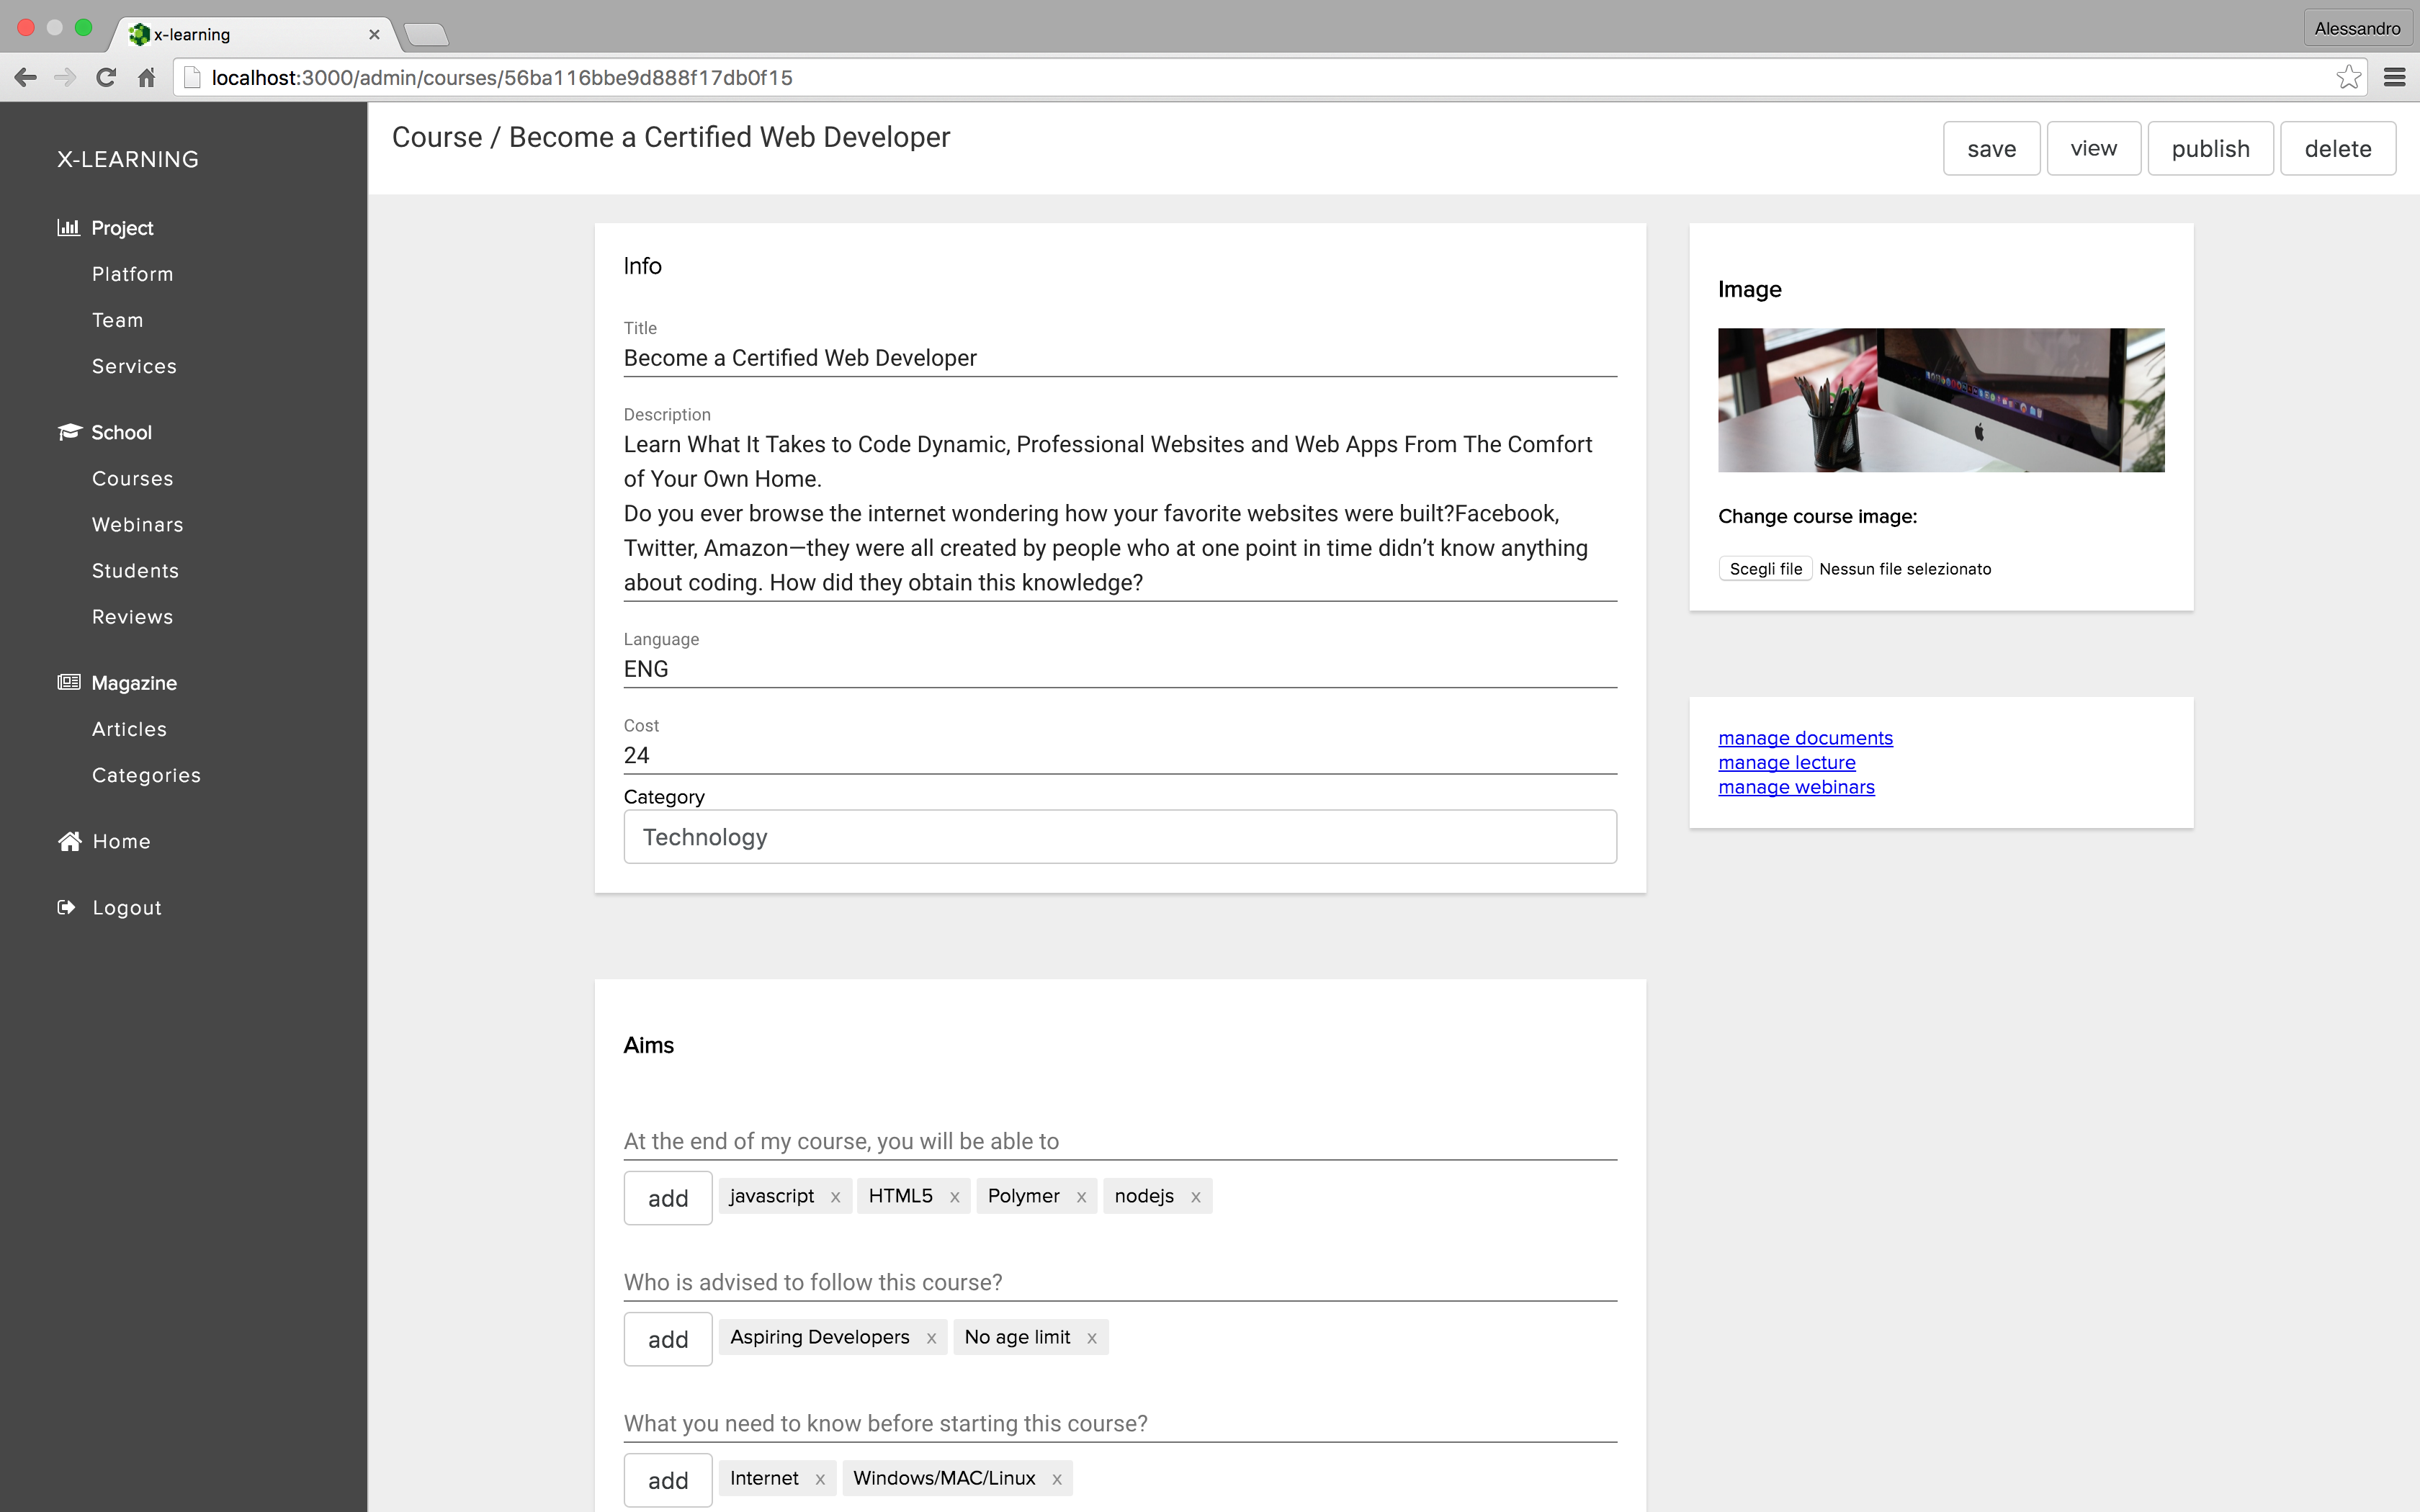
\includegraphics[width=1.0\linewidth]{images/chapter4/page-course-admin.png}
    \captionof{figure}[page course admin]{page course admin}
\end{minipage}

\item \textbf{page lecture} L'immagine seguente rappresenta la page lecture dove il teacher può gestire la creazione e la modifica di tutte le informazioni della singola lecture\par

\begin{minipage}{\linewidth}
    \centering
    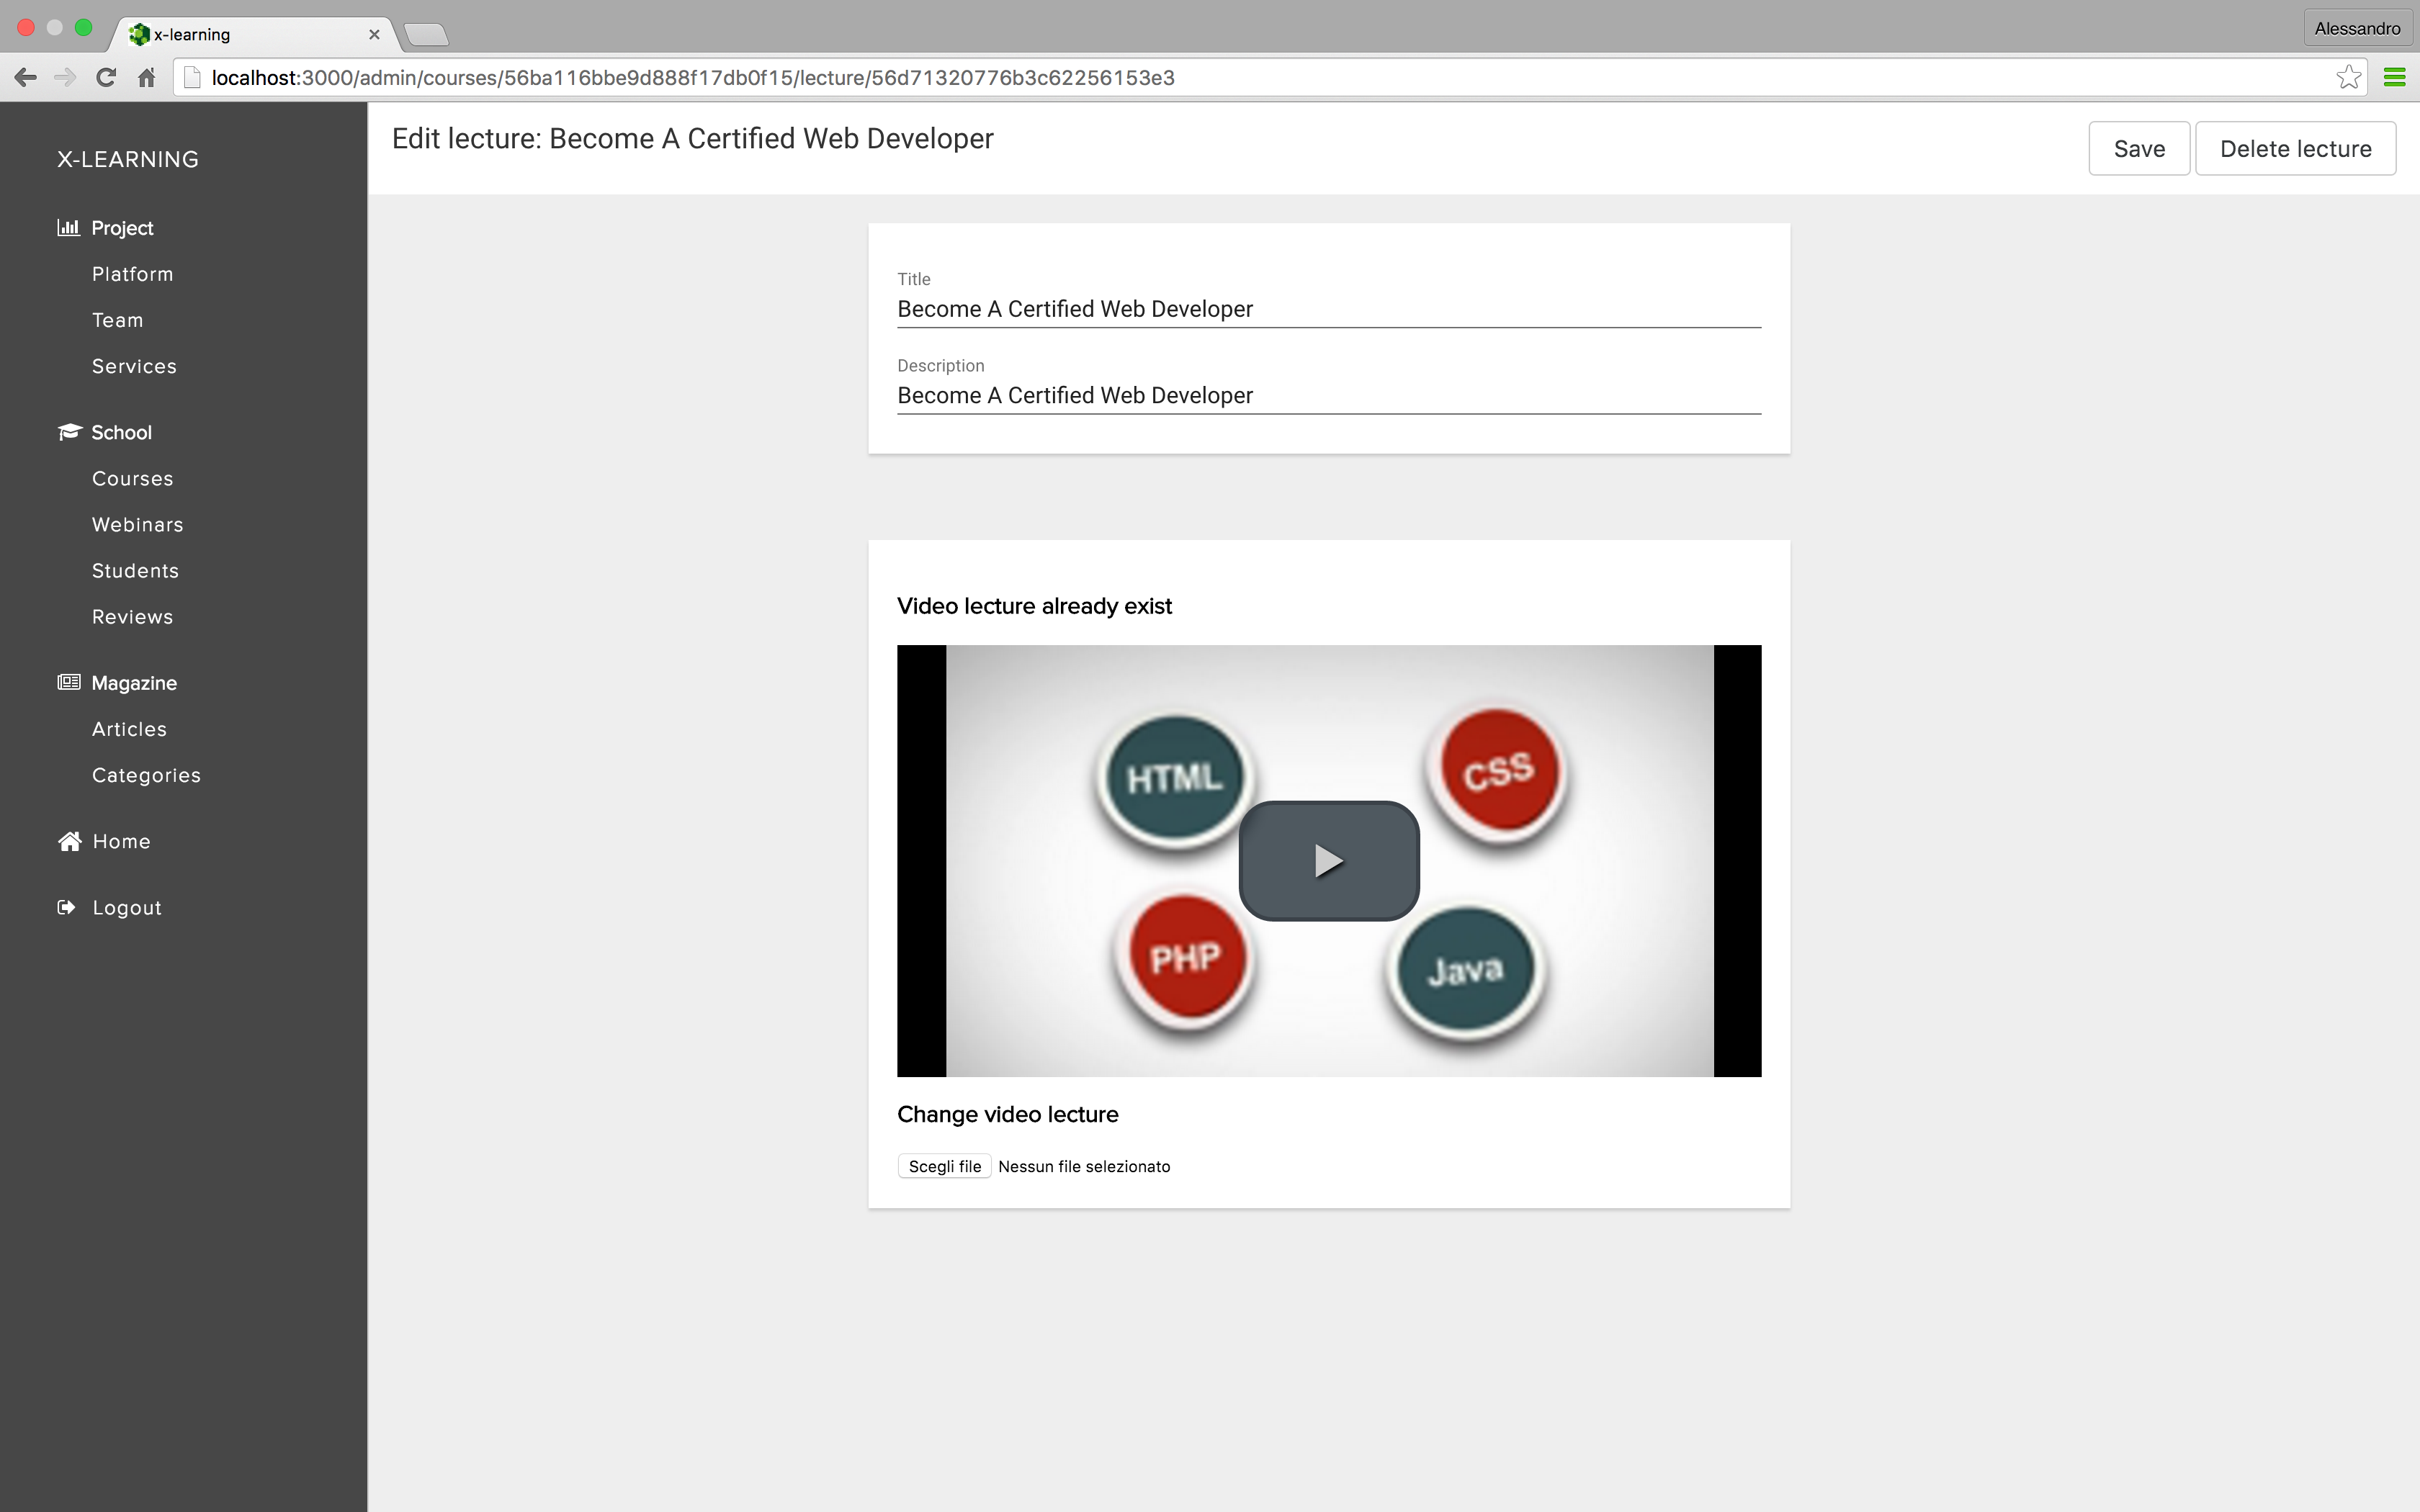
\includegraphics[width=1.0\linewidth]{images/chapter4/page-lecture-admin.png}
    \captionof{figure}[page lecture admin]{page lecture admin}
\end{minipage}

\item \textbf{page webinar} L'immagine seguente rappresenta la page lecture dove il teacher può gestire la creazione e la modifica di tutte le informazioni di un singolo webinar\par

\begin{minipage}{\linewidth}
    \centering
    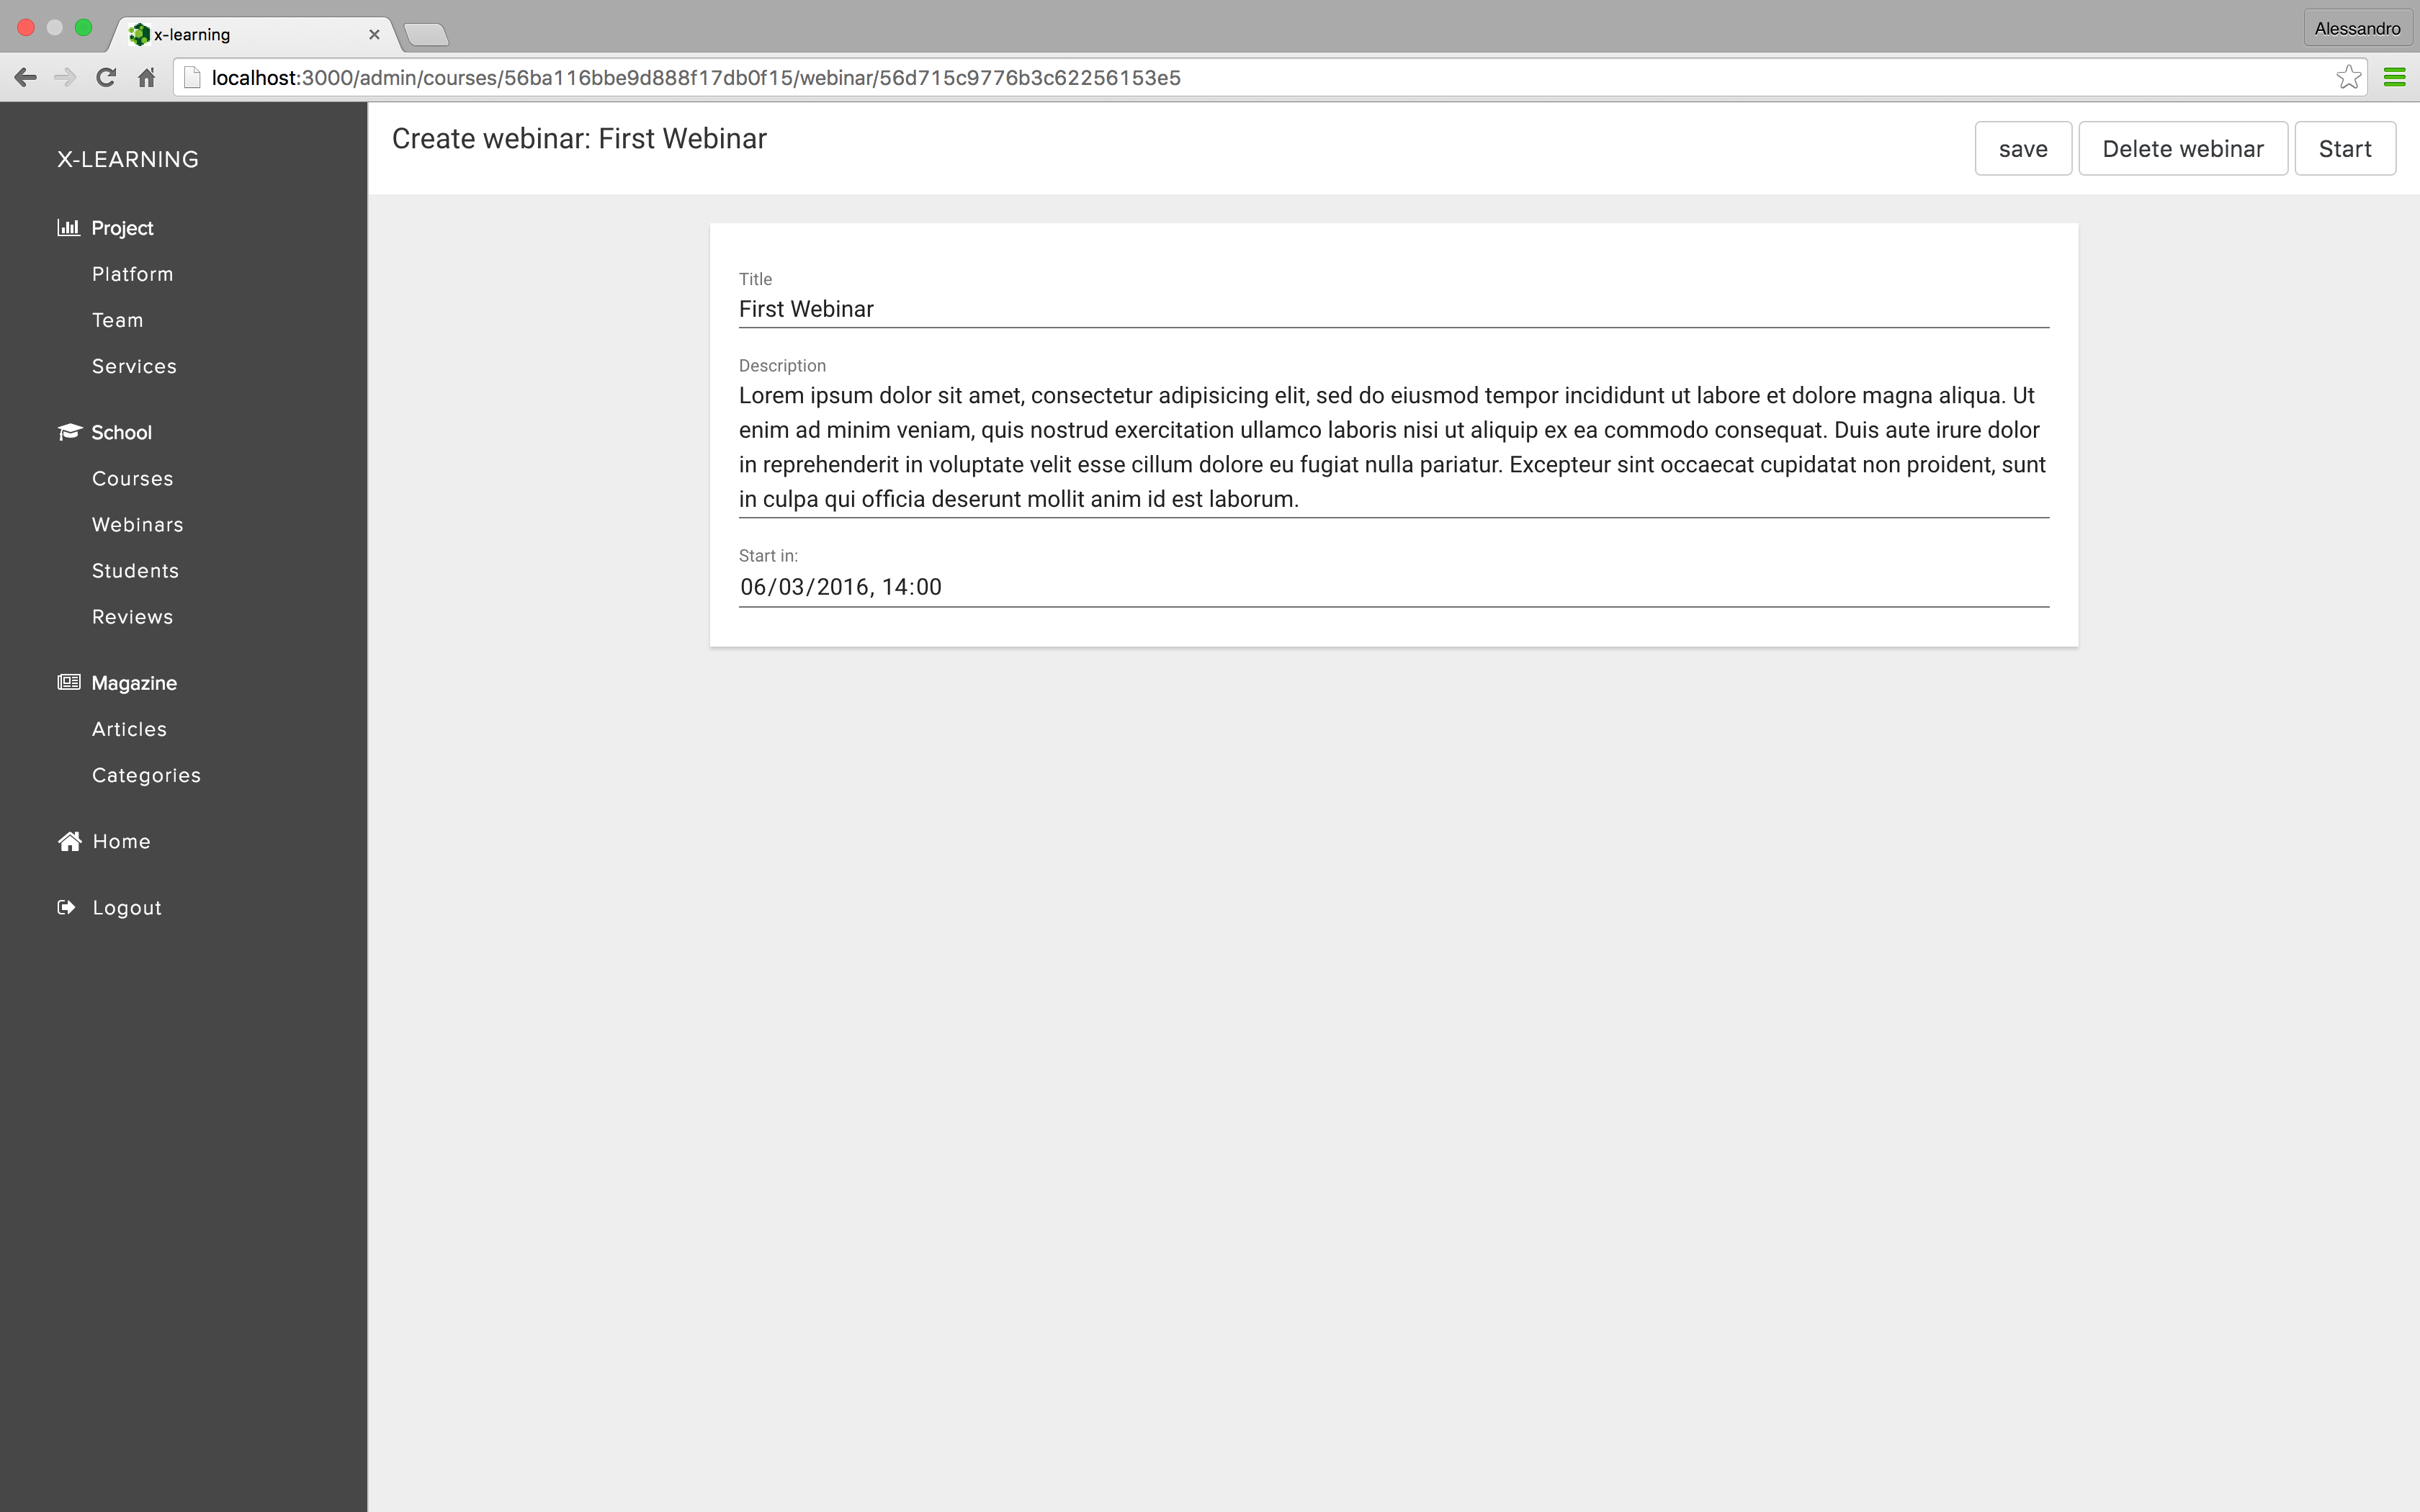
\includegraphics[width=1.0\linewidth]{images/chapter4/page-webinar-admin.png}
    \captionof{figure}[page webinar admin]{page webinar admin}
\end{minipage}

\end{itemize}


\subsubsection {Client side}
\label{subsec:Client_side}
The client side is the part of the platform that allows users to view courses and then attend lectures, webinars and access to educational materials.
The main pages that compose the client side are:

\begin{itemize}

\item \textbf{page home} L'immagine seguente rappresenta la Page Home dove lo student può cercare un determinato corso, vedere quelli disponibili, e eventualmente filtrari per categoria\par

\begin{minipage}{\linewidth}
    \centering
    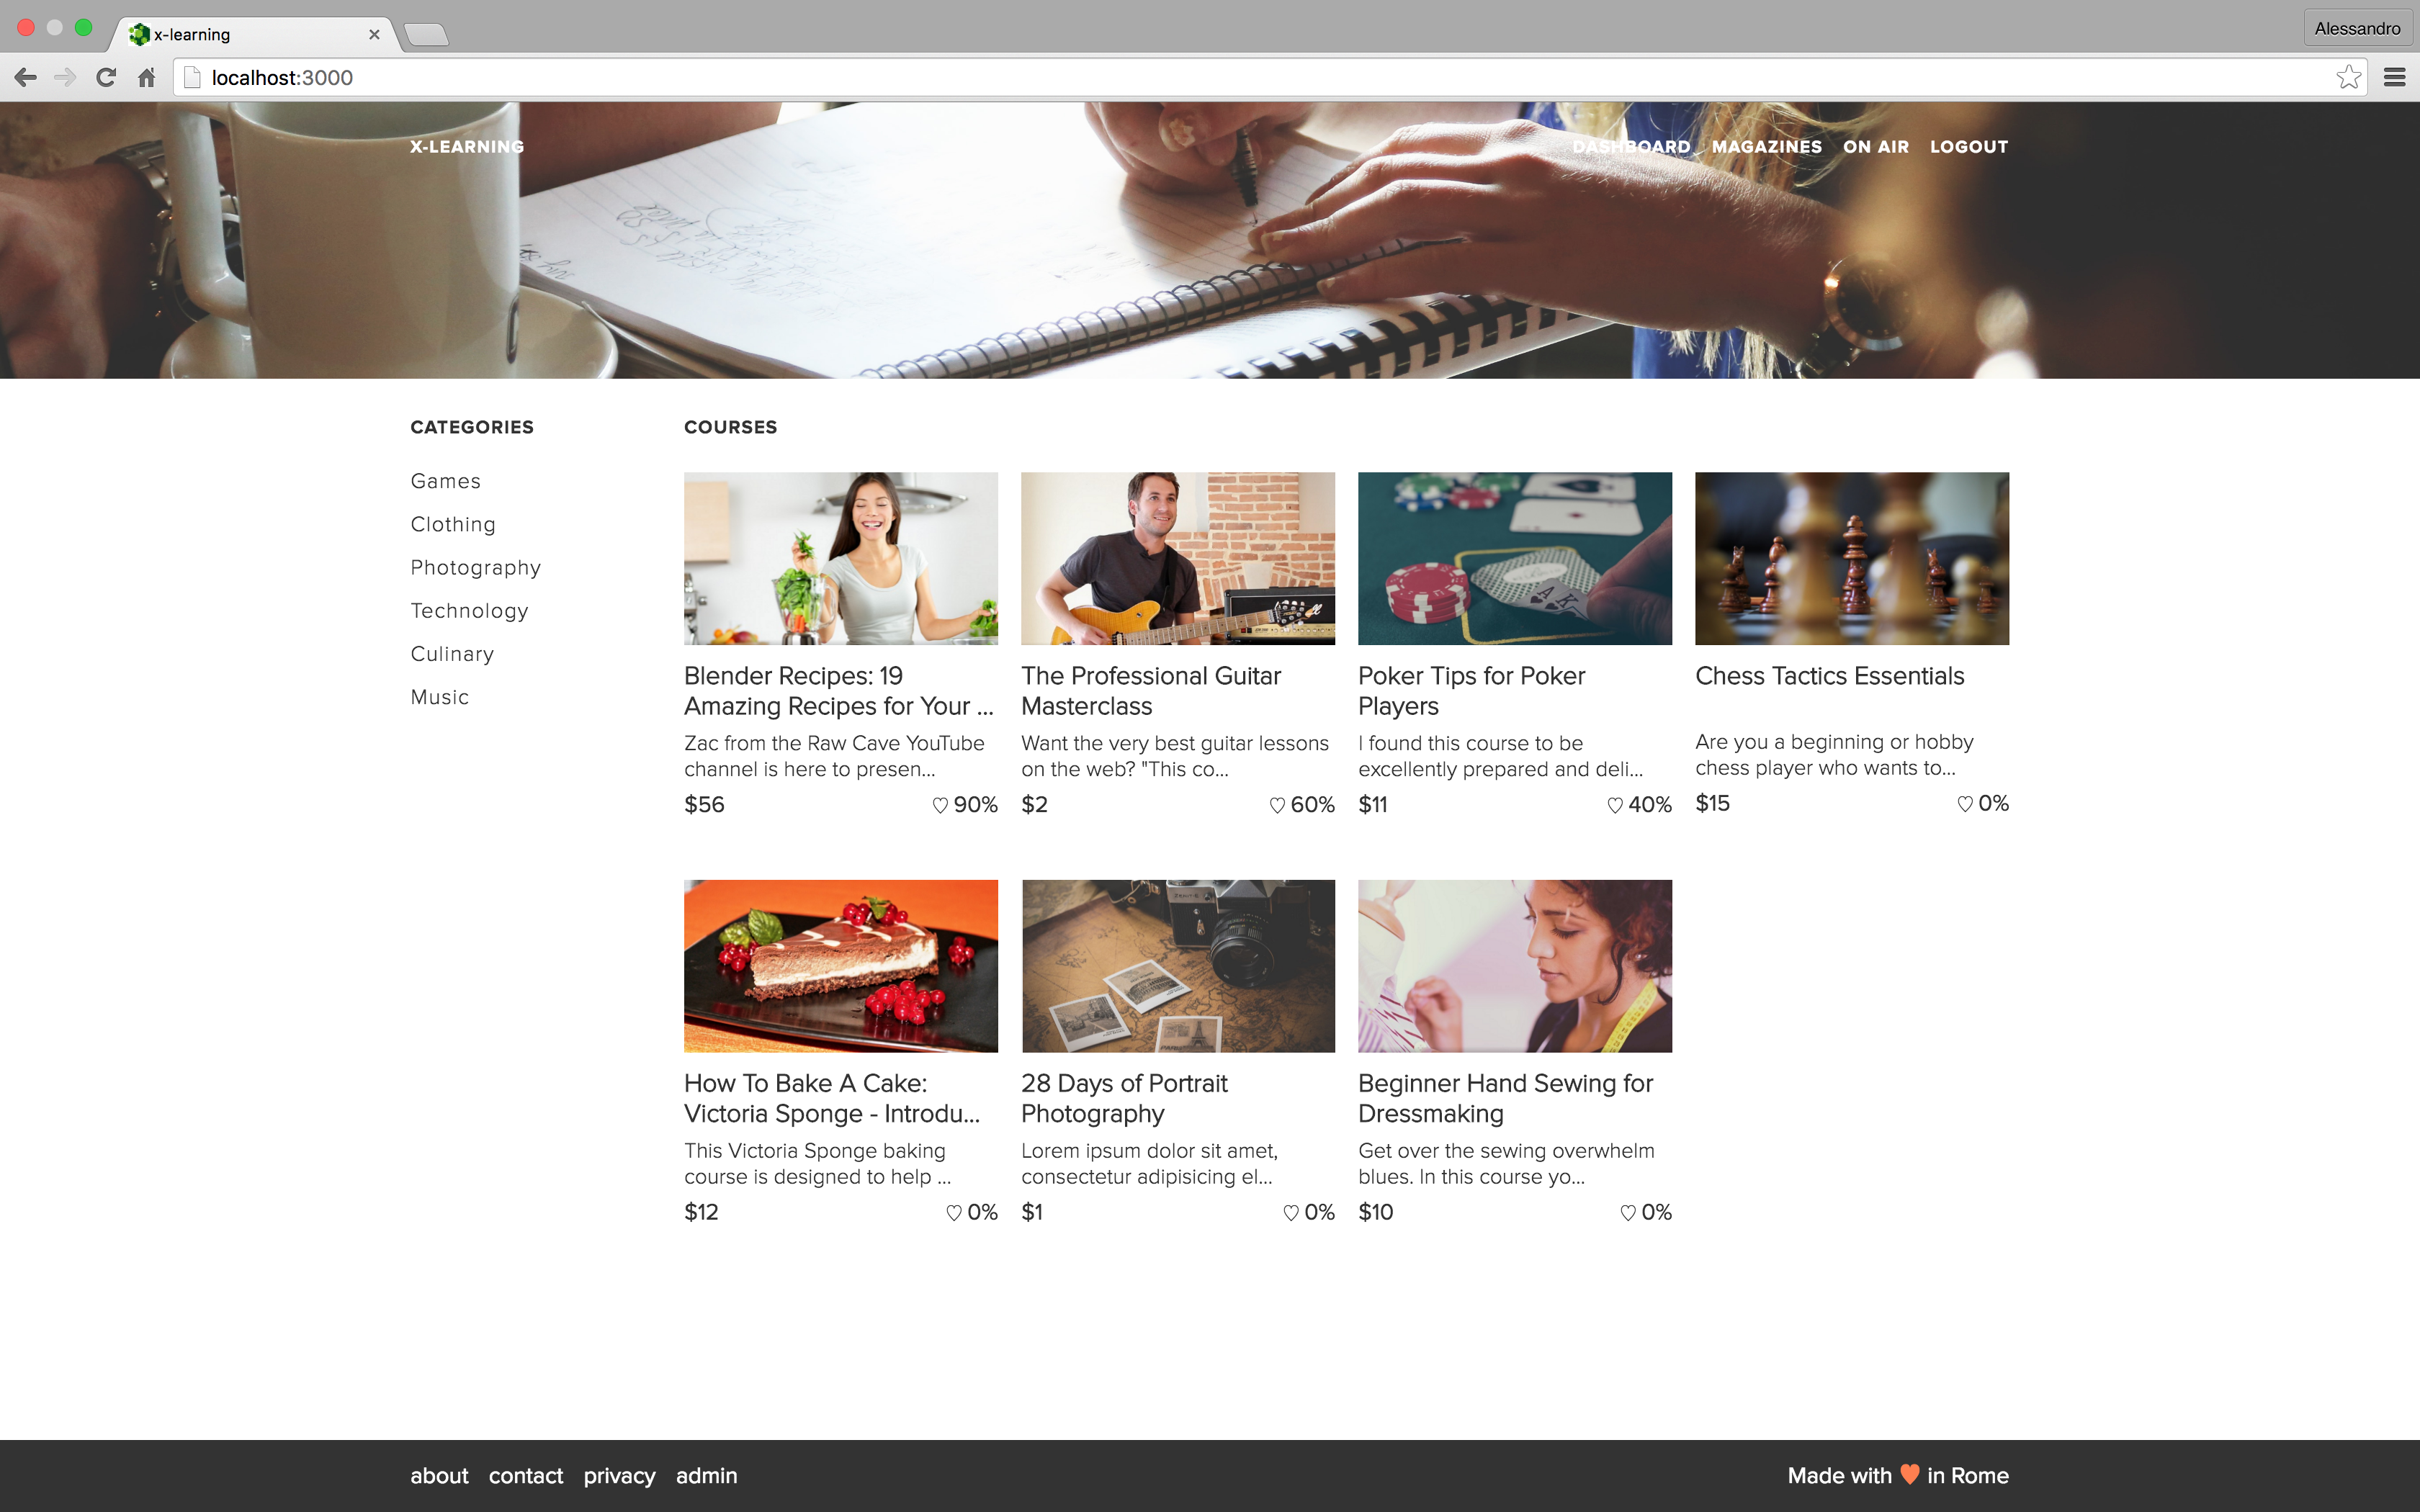
\includegraphics[width=1.0\linewidth]{images/chapter4/page-home.png}
    \captionof{figure}[page home]{page home}
\end{minipage}


\item \textbf{page course} L'immagine seguente rappresenta la Page Course dove è possibile trovare tutte le informazioni di un singolo corso come costo, review, video lezioni, materiale didattico \par
\begin{minipage}{\linewidth}
    \centering
    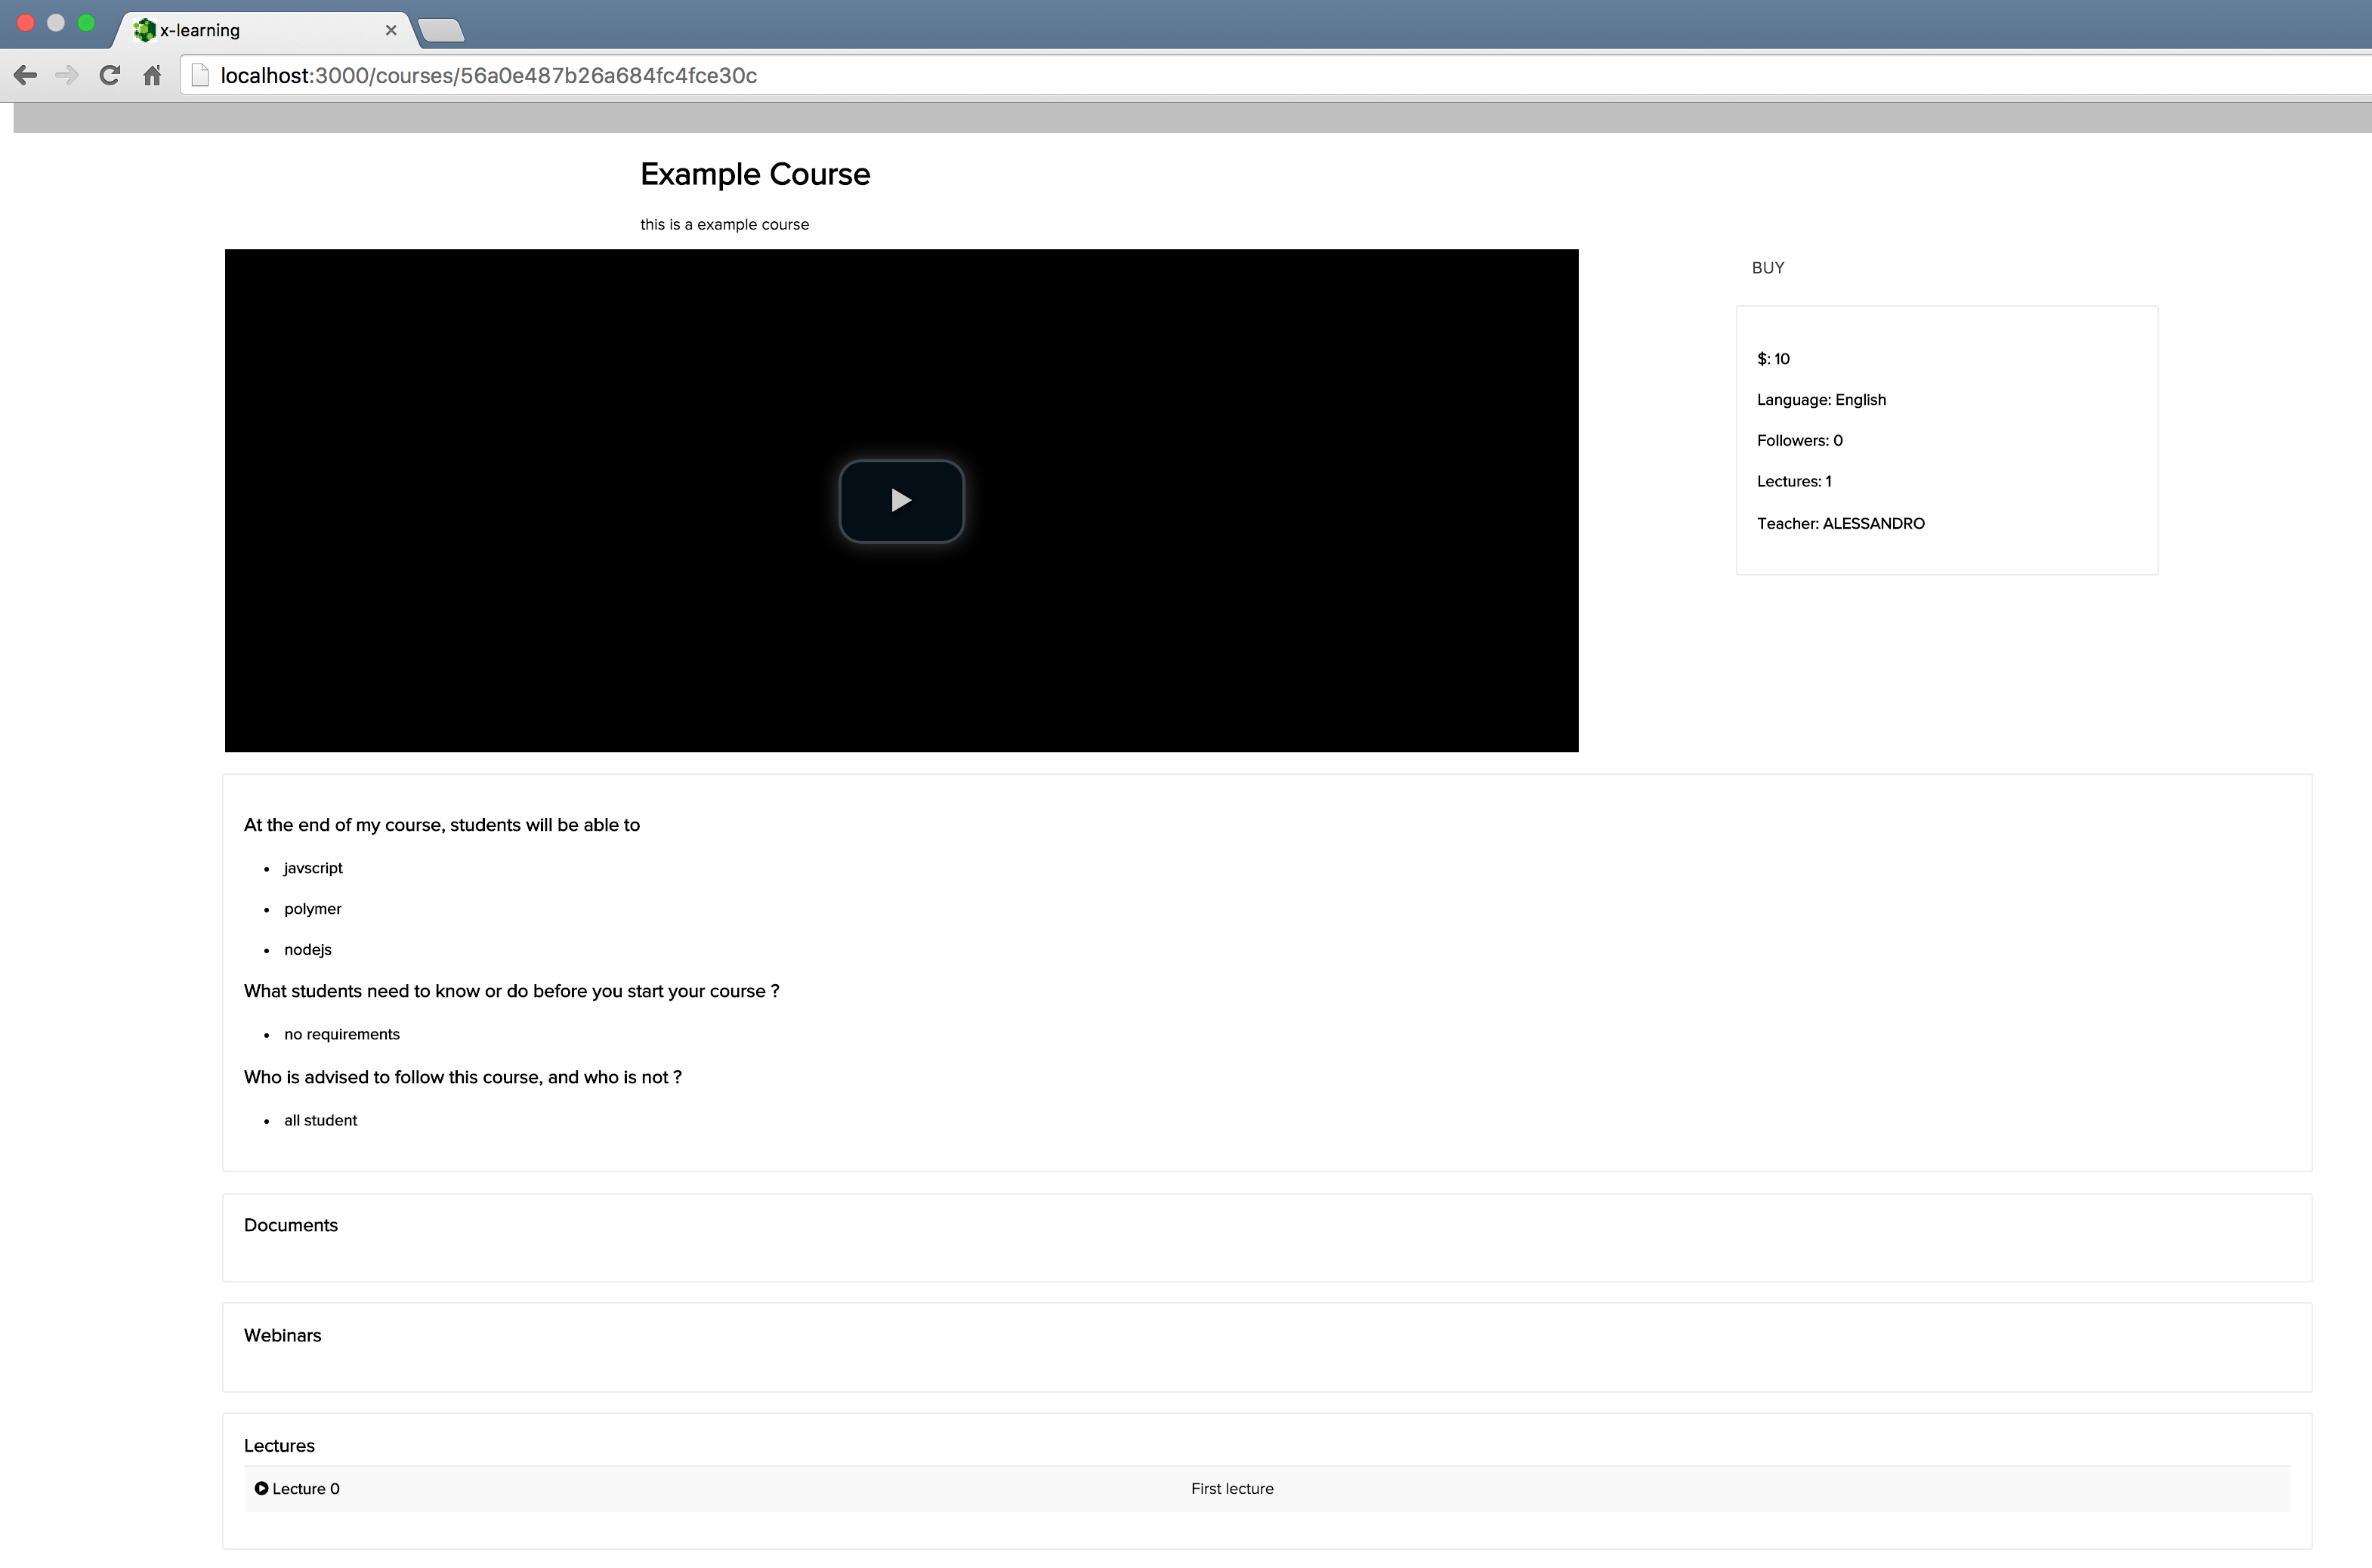
\includegraphics[width=1.0\linewidth]{images/chapter4/page-course.png}
    \captionof{figure}[page course]{page course}
\end{minipage}


\item \textbf{page lecture} L'immagine seguente rappresenta la Page lecture che permette la visualizzazione della video lezione\par

\begin{minipage}{\linewidth}
    \centering
    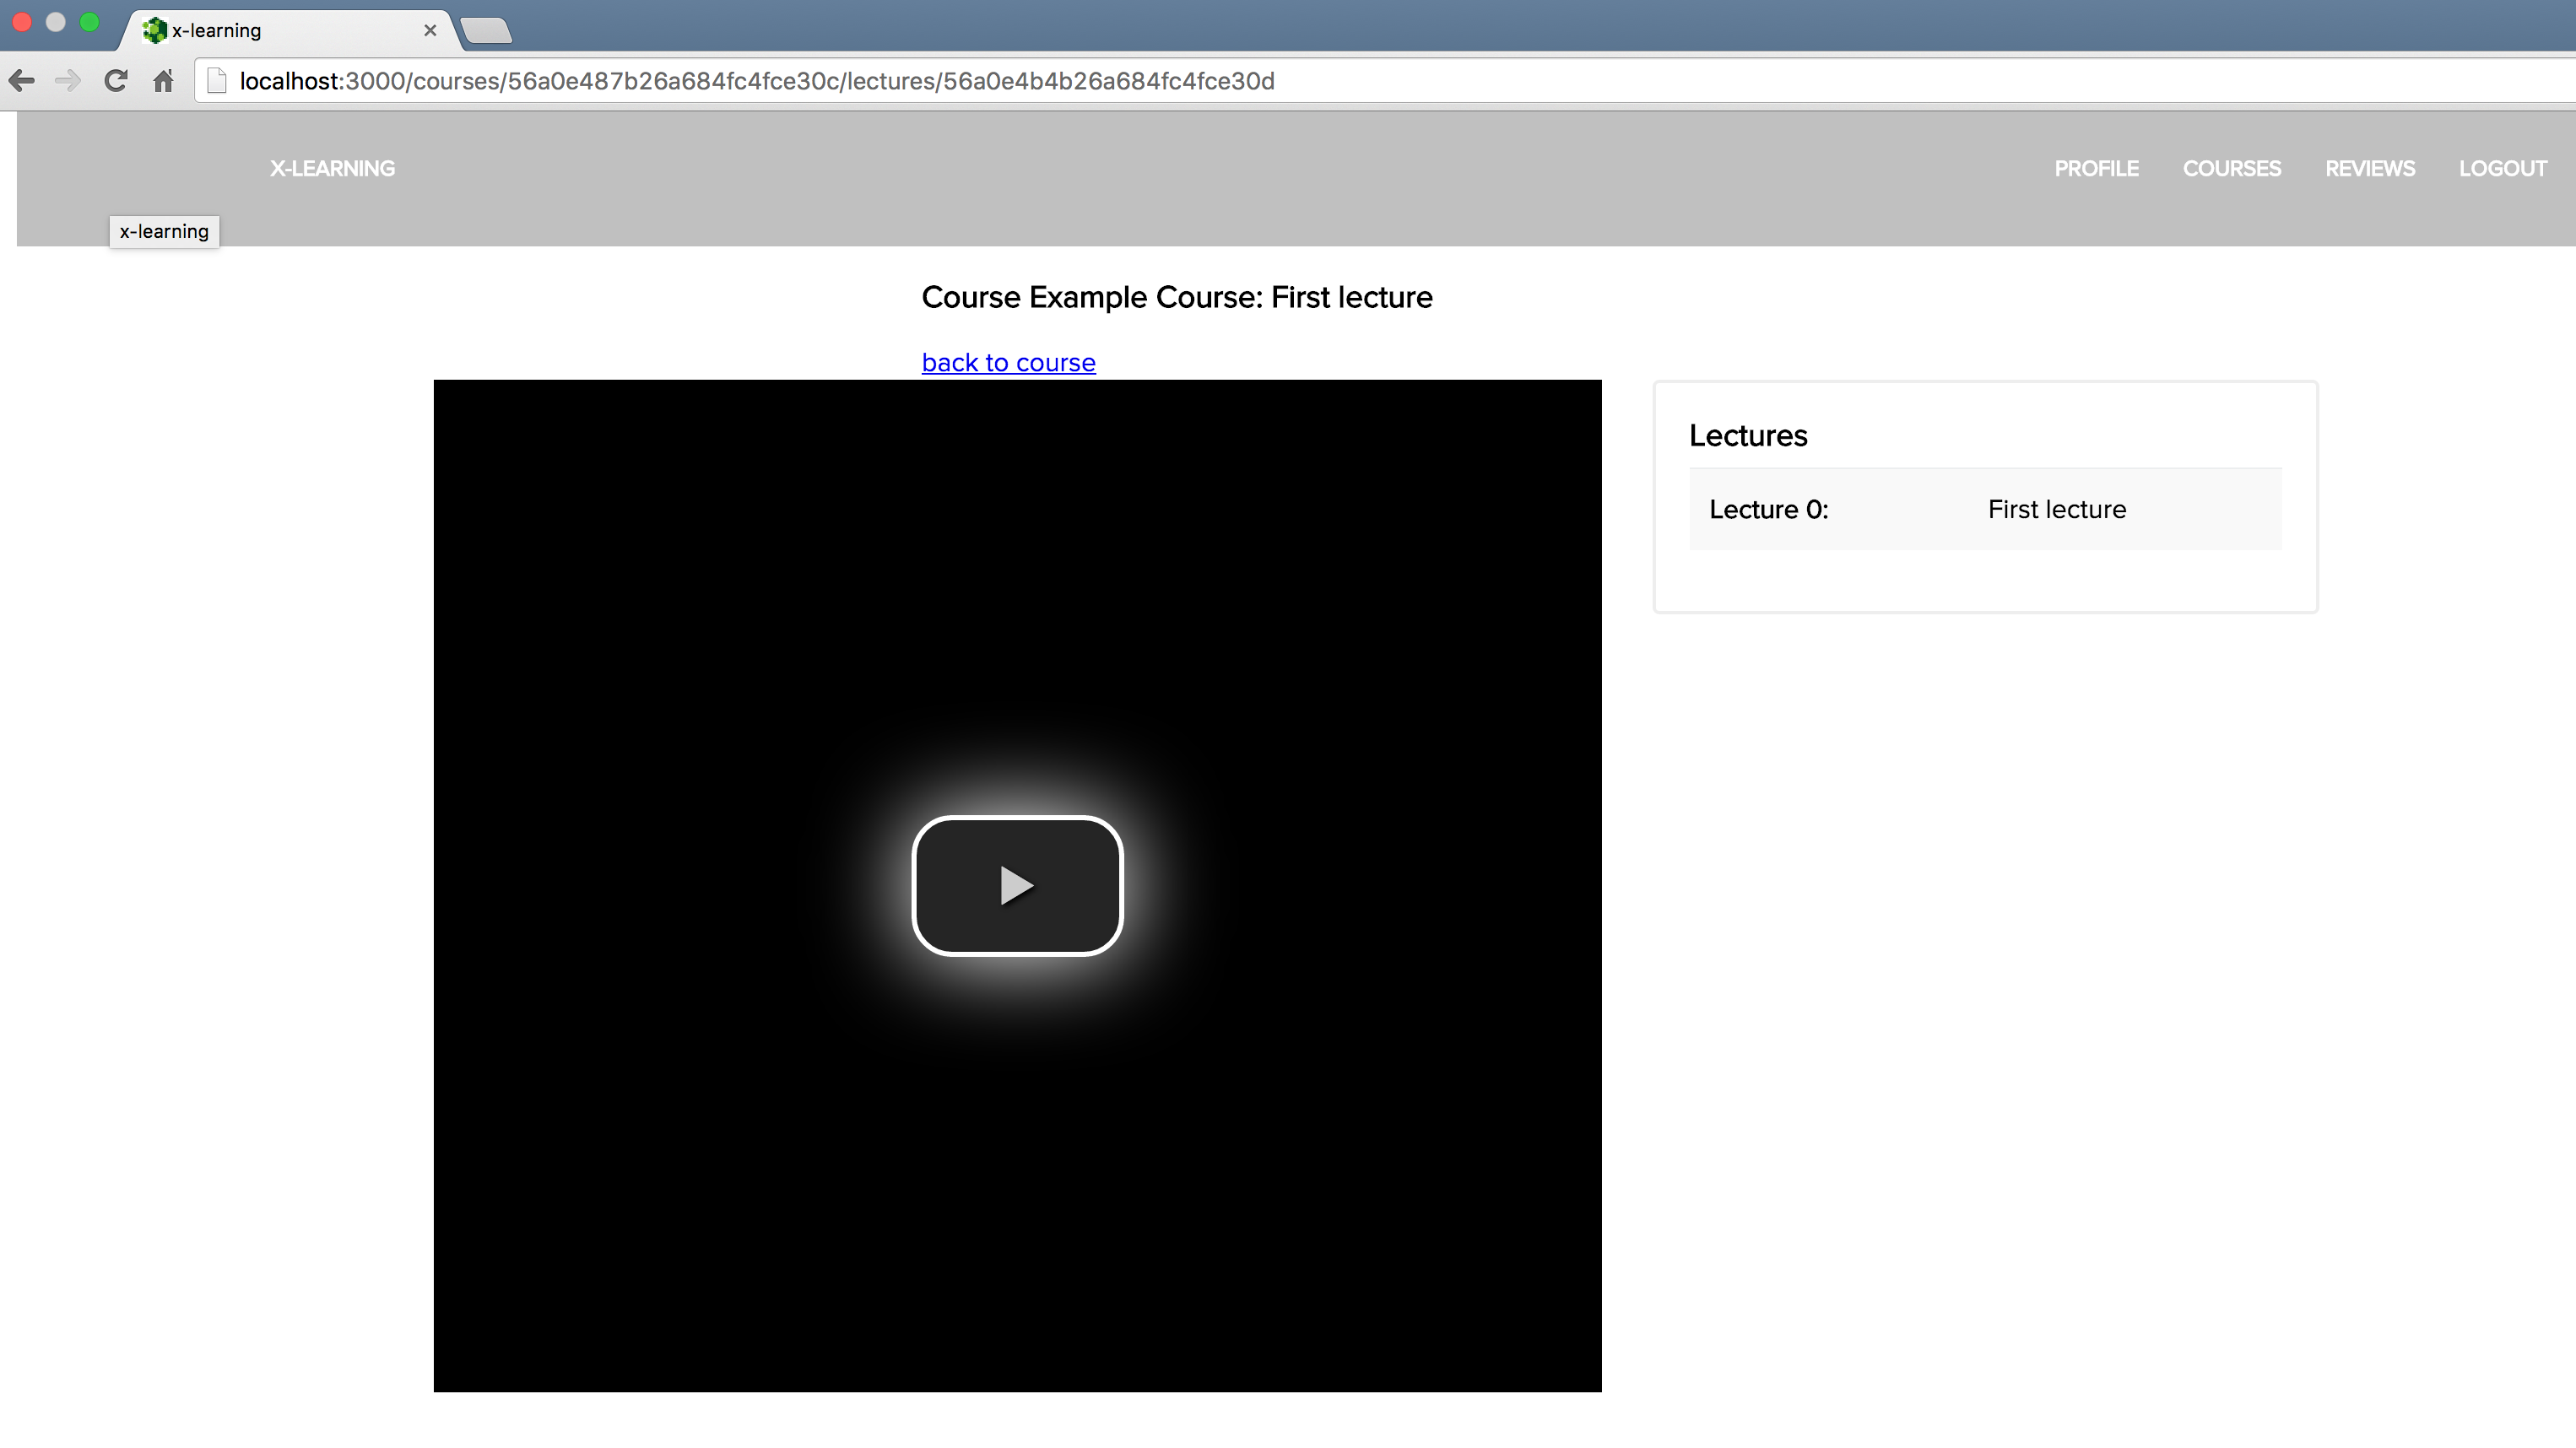
\includegraphics[width=1.0\linewidth]{images/chapter4/page-lecture.png}
    \captionof{figure}[page lecture]{page lecture}
\end{minipage}


\item \textbf{page webinar} L'immagine seguente rappresenta la Page Webinar che permette di collegarsi in tempo reale al webinar di un determianto corso\par
\begin{minipage}{\linewidth}
    \centering
    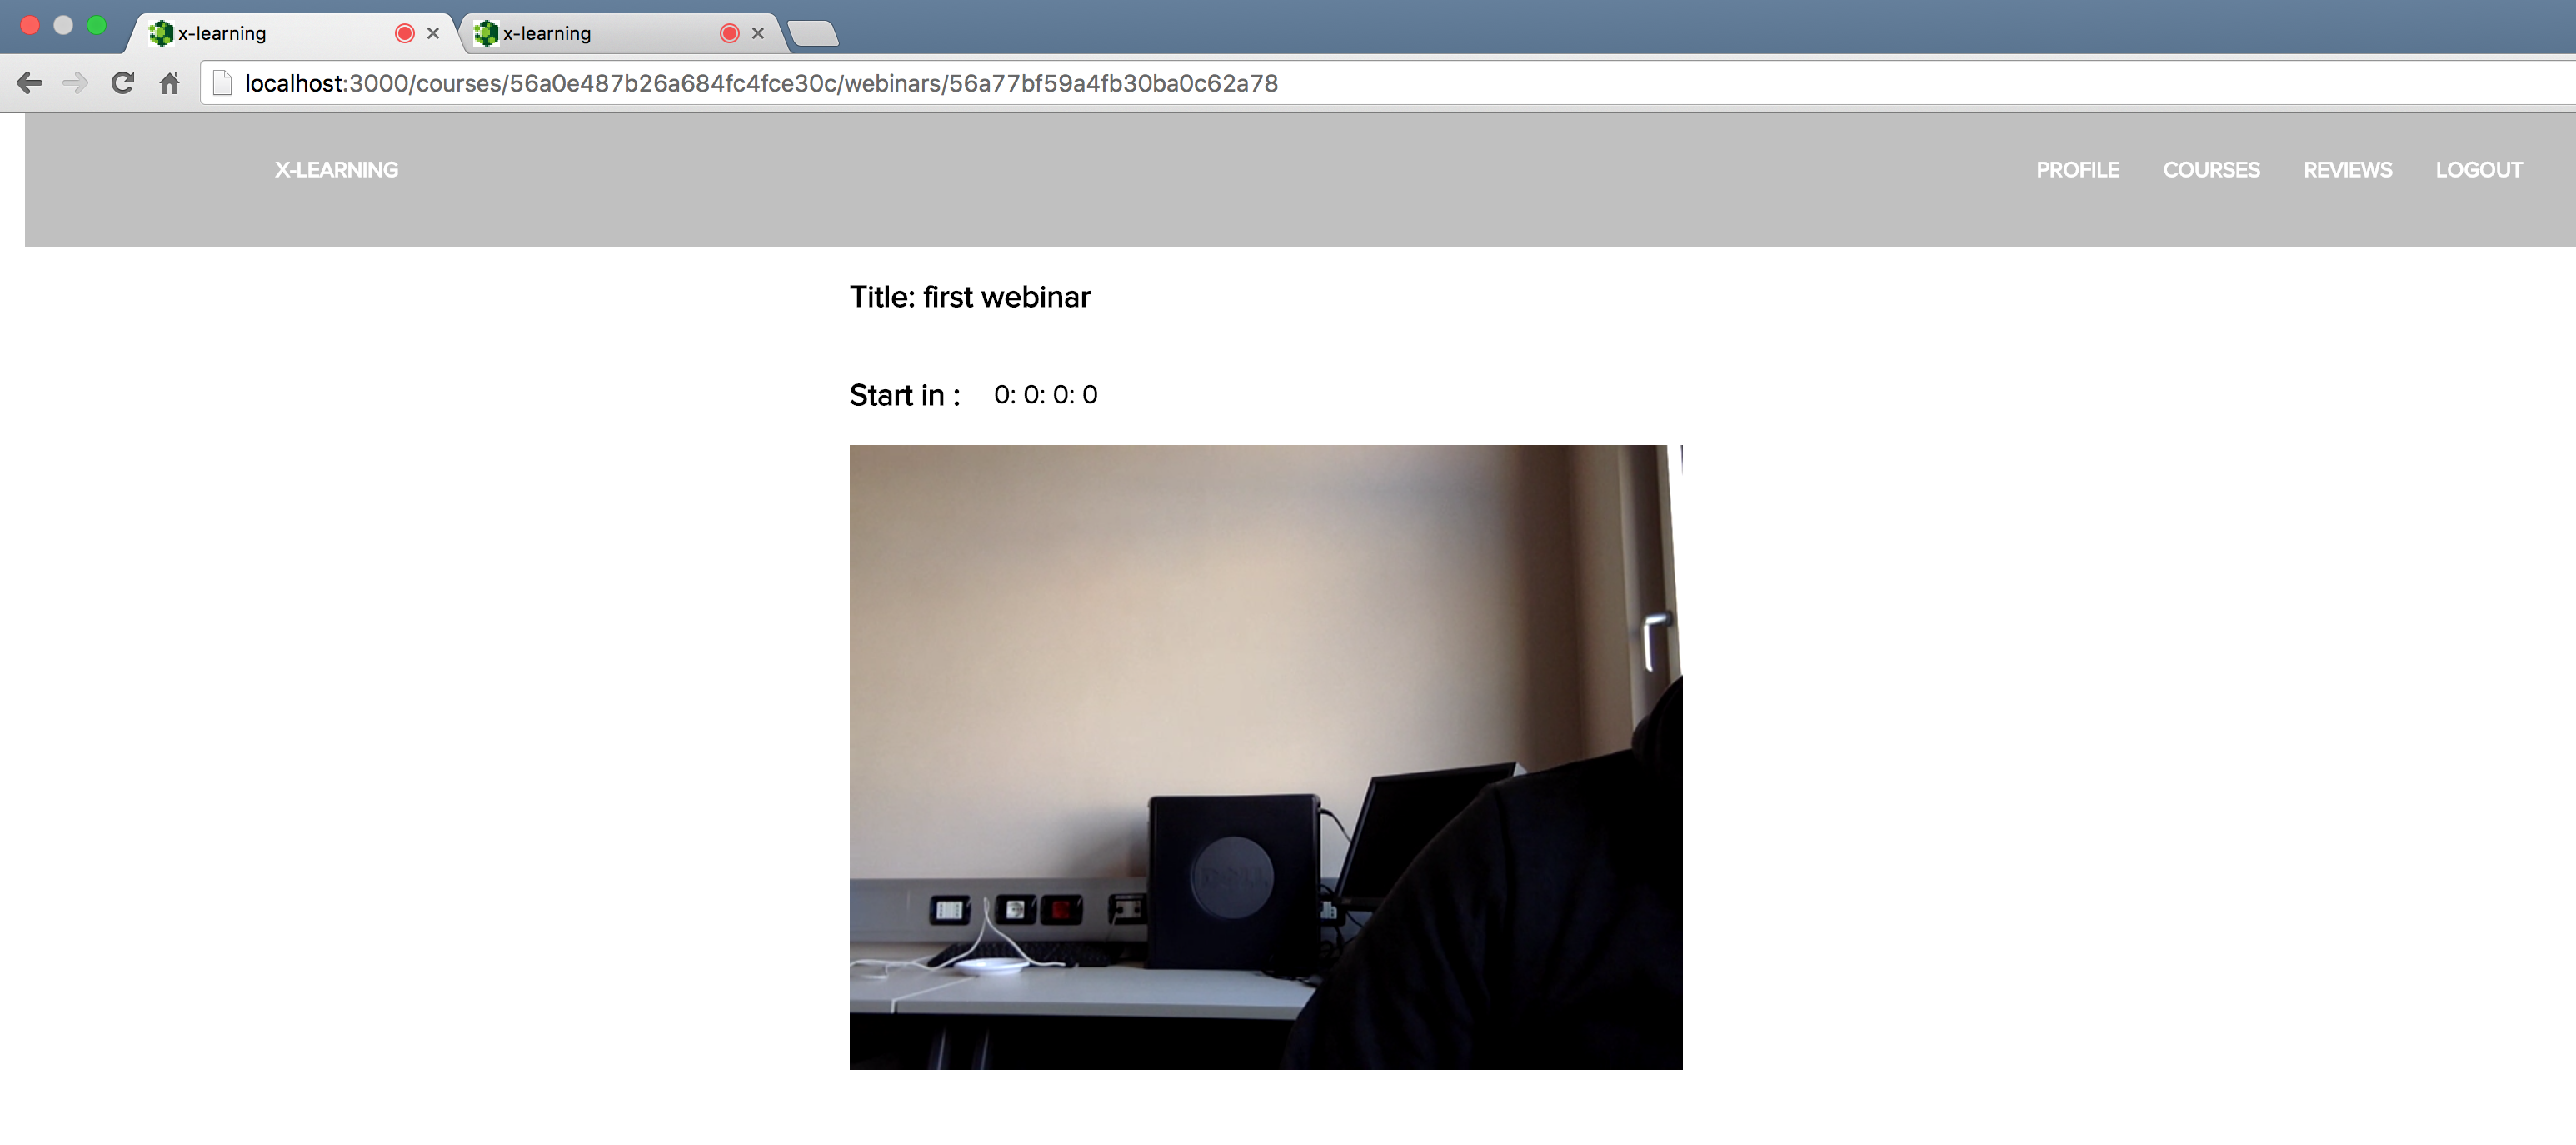
\includegraphics[width=1.0\linewidth]{images/chapter4/page-webinar.png}
    \captionof{figure}[page webinar]{page webinar}
\end{minipage}

\end{itemize}



\subsubsection { UI components assembly}
\label{subsec:4th_step_UI_components_assembly}

Distinct UI components are finally mounted to compose the application views. Assembly is kept as simple as possible: it only consists of a composition of HTML5 elements. So, the entire development process results driven by: JSON documents describing entities of the application and HTML template documents describing the UI components.
{\color{red} The following is an example: }

\begin{figure}[htb] %  figure placement: here, top, bottom
 \centering
 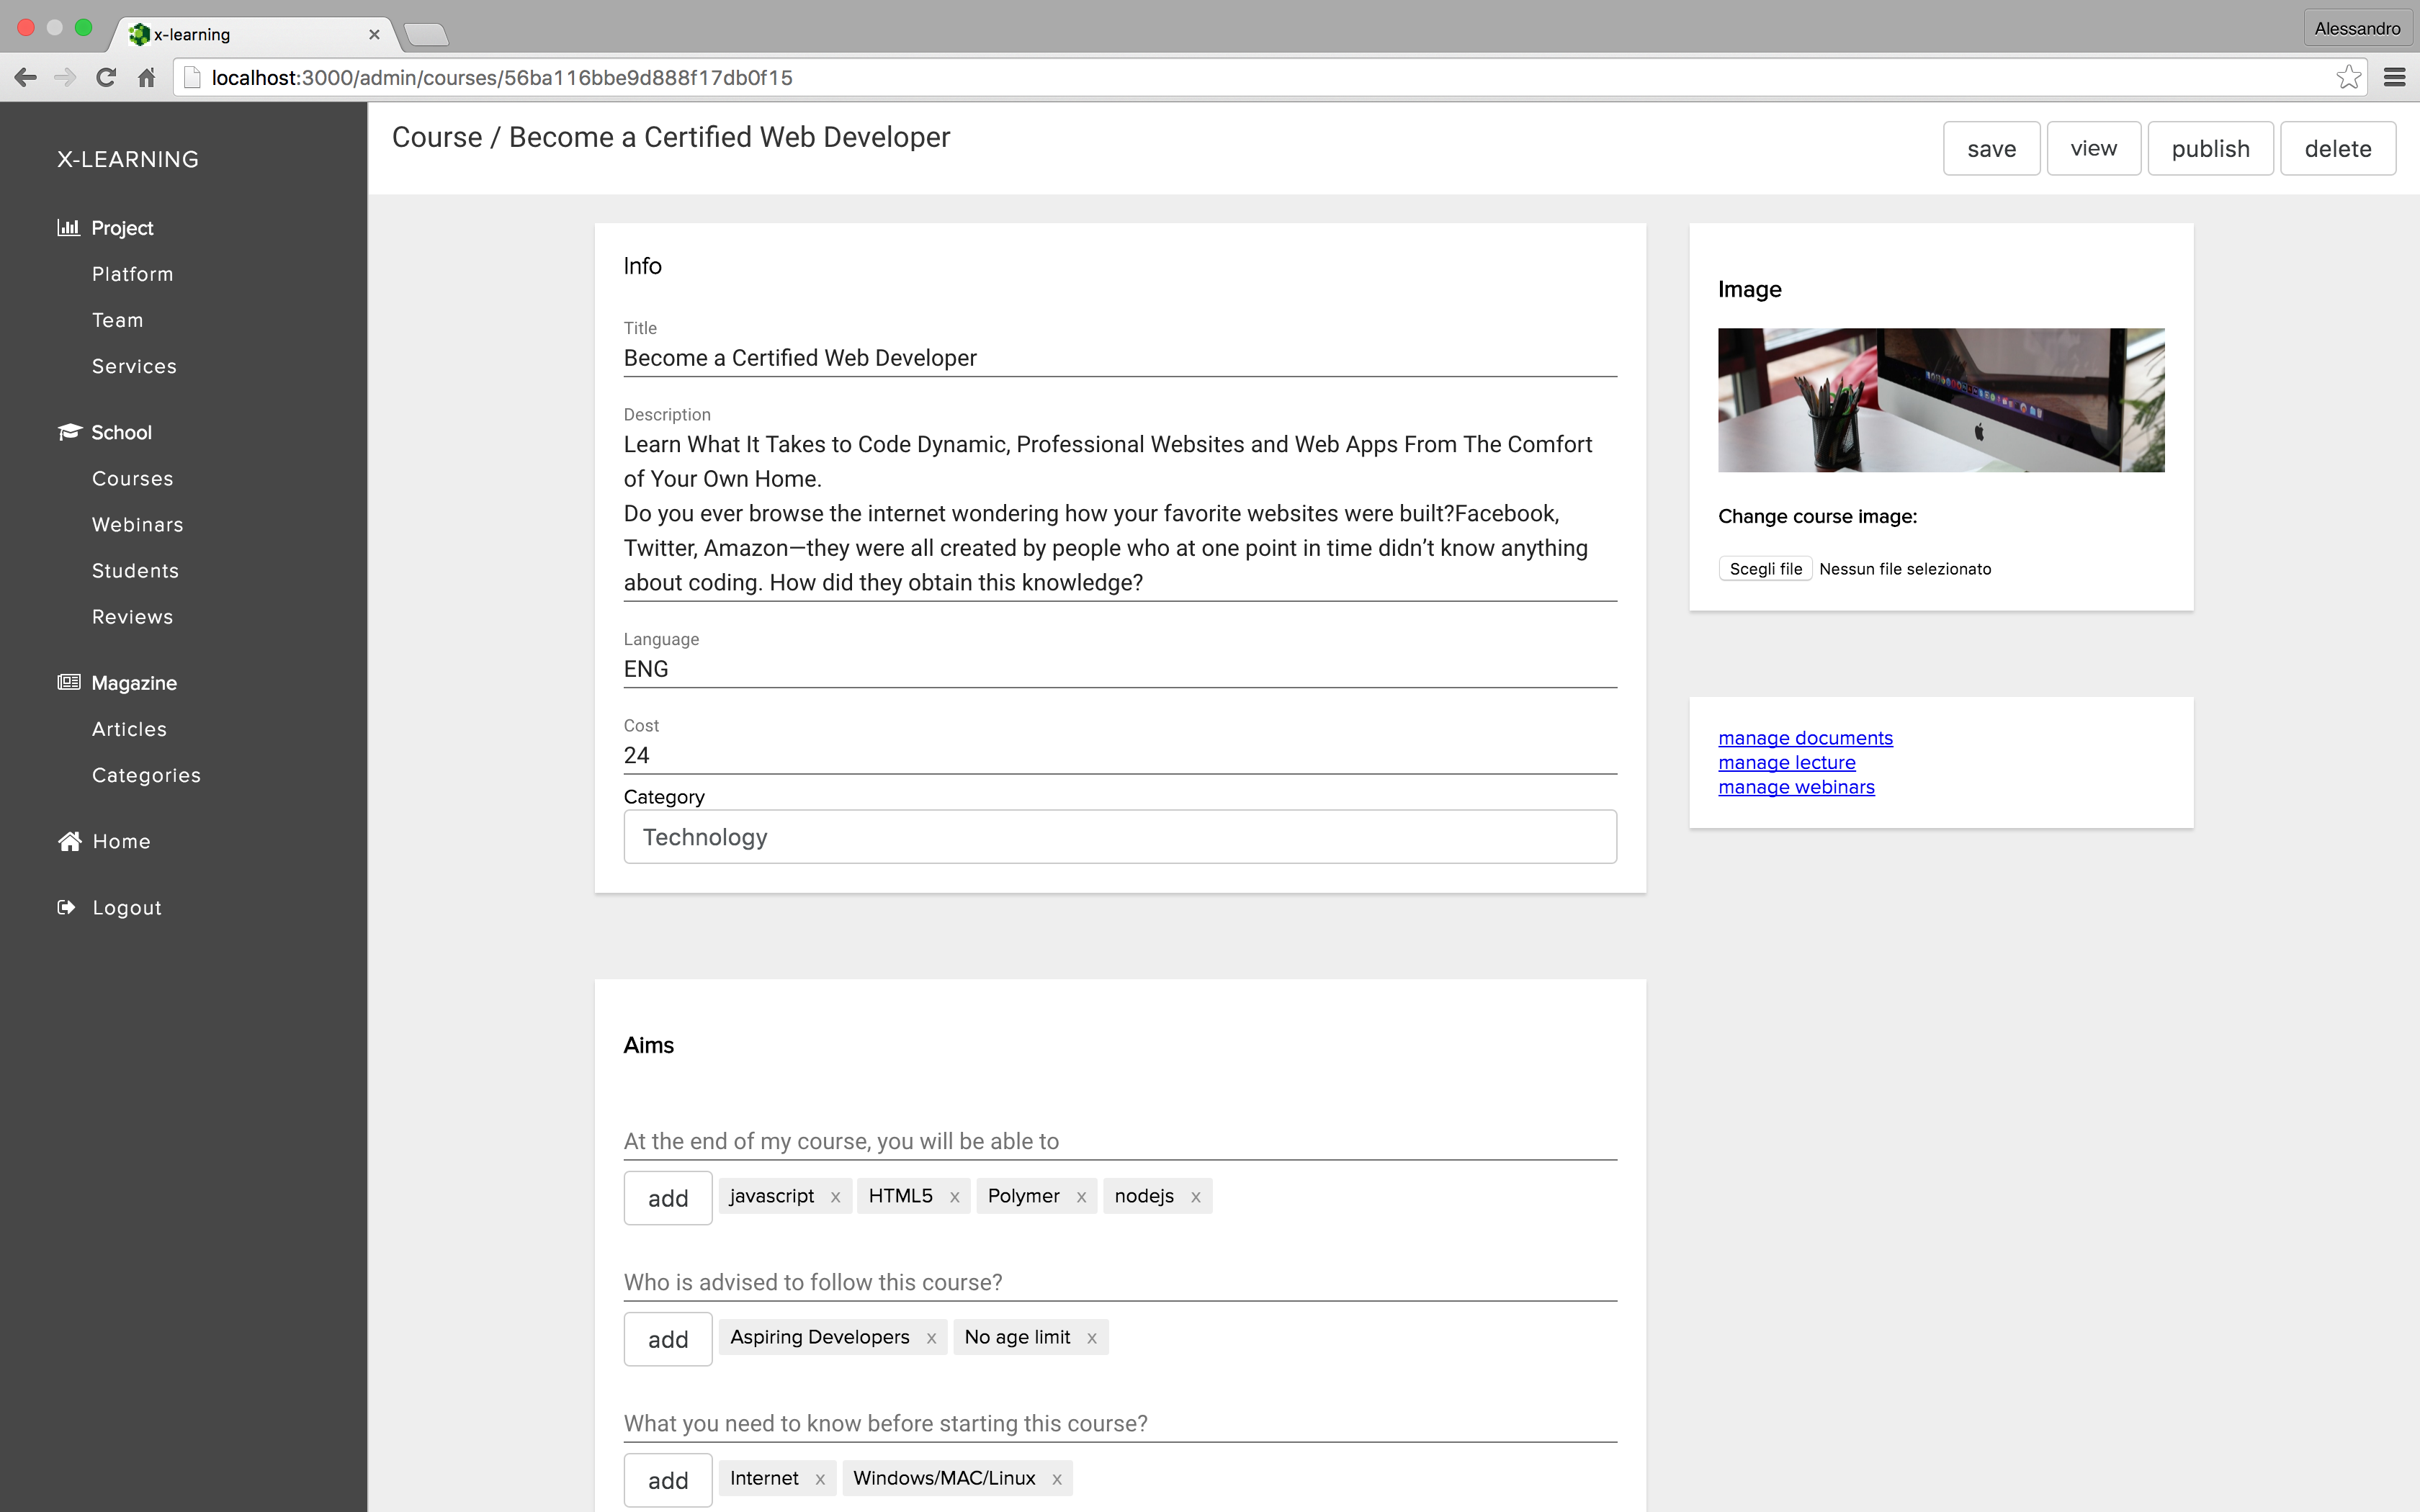
\includegraphics[width=1.0\linewidth]{images/chapter4/page-course-admin.png}\hfill
 \caption[Page Admin course action]{Page Admin course action}
 \label{fig:fourV}
\end{figure}

In the image below shows the edit page of the course composed of the following Web component:

\begin{lstlisting}[language=html]
<part-course-actions course="{{course}}"></part-course-actions>
\end{lstlisting}


\begin{figure}[htb] %  figure placement: here, top, bottom
 \centering
 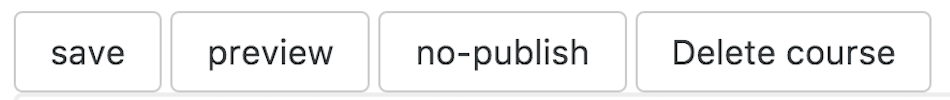
\includegraphics[width=1.0\linewidth]{images/chapter4/admin-course-actions.png}\hfill
 \caption[Page Admin course action]{Page Admin course action}
 \label{fig:fourV}
\end{figure}

\begin{lstlisting}[language=html]
<part-course-info course="{{course}}" error="{{error}}"></part-course-info>
\end{lstlisting}



\begin{minipage}{\linewidth}
    \centering
    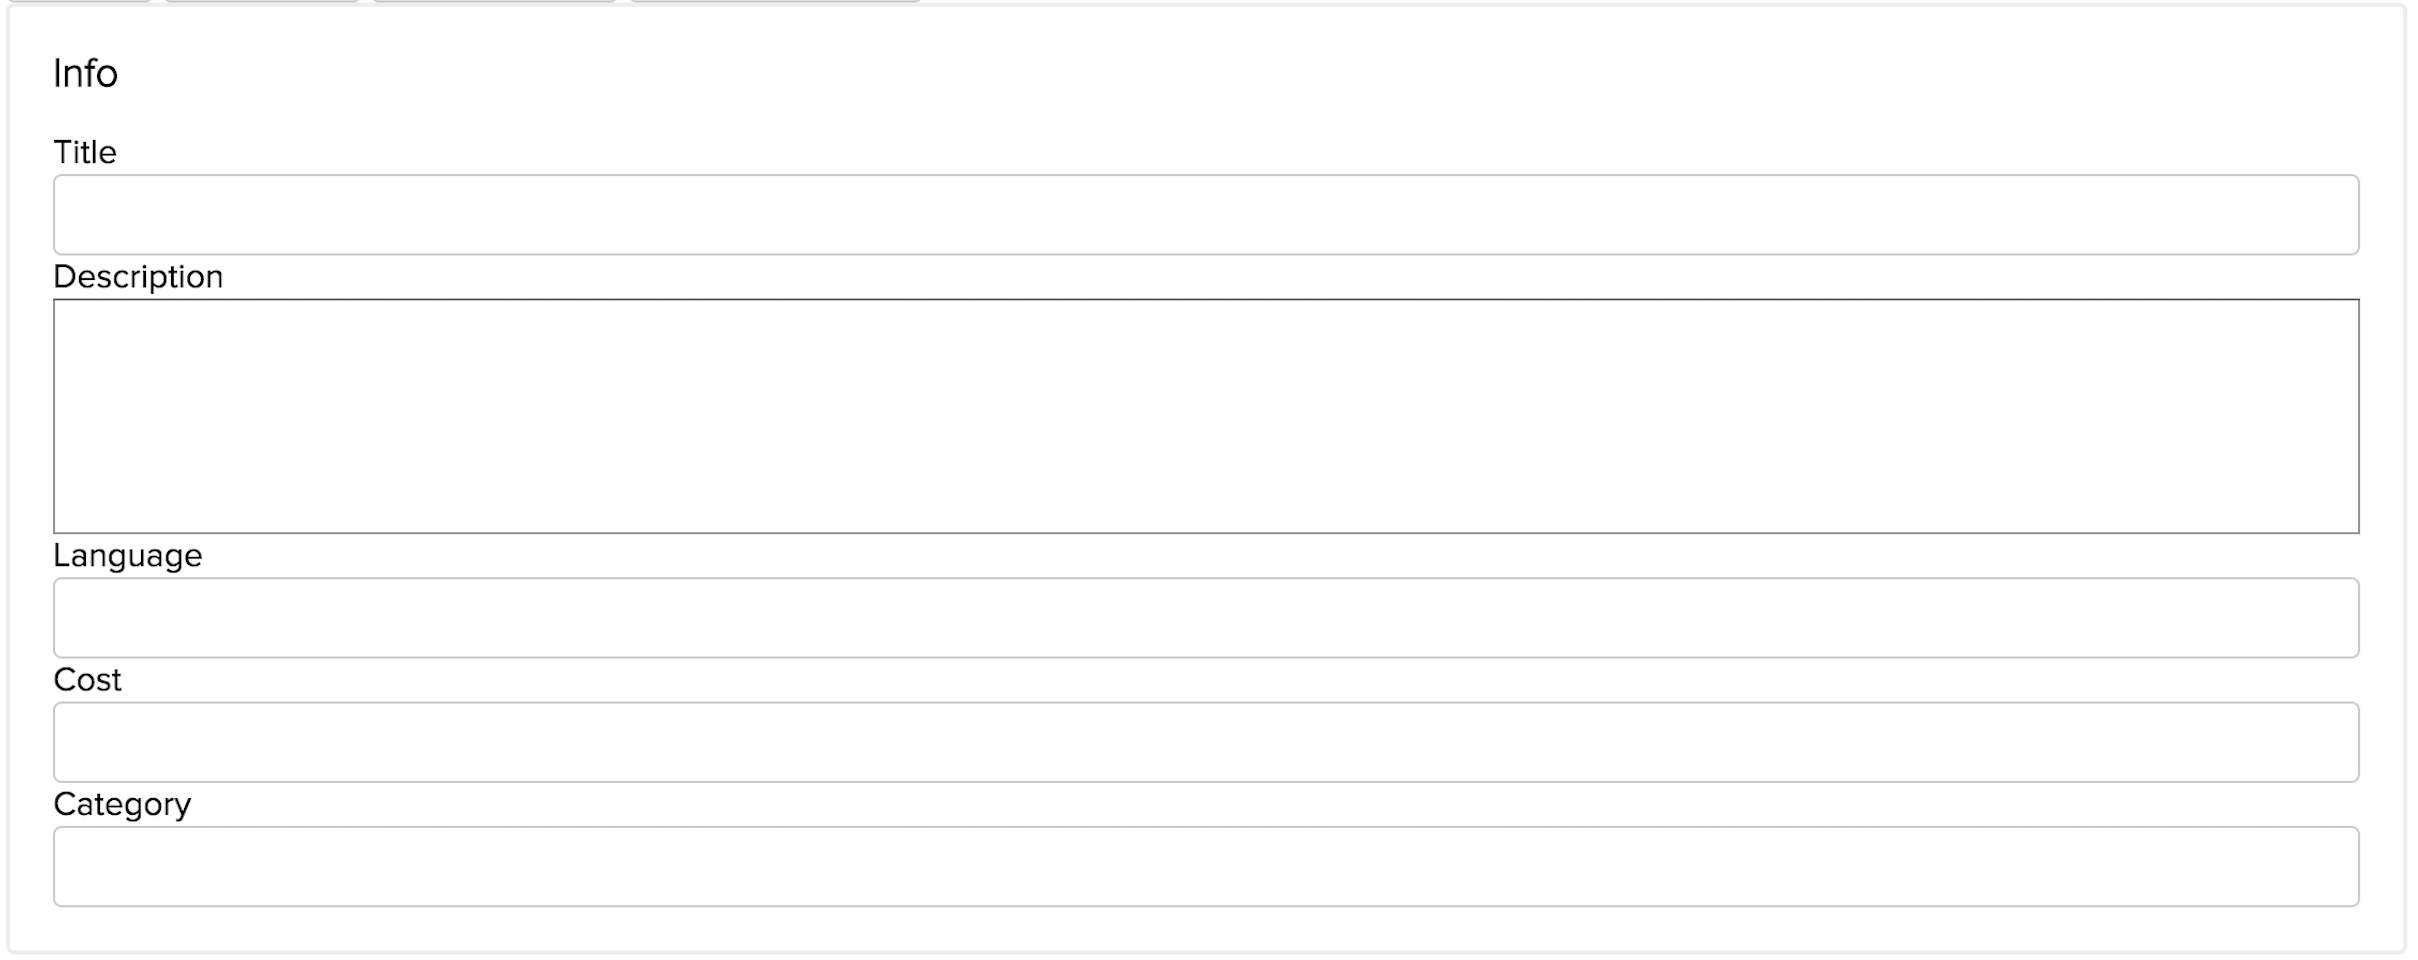
\includegraphics[width=1.0\linewidth]{images/chapter4/admin-course-info.png}
    \captionof{figure}[Page Admin course info]{Page Admin course info}
\end{minipage}

Also as you can see on the page is given the opportunity to manage the different components of the course:
\begin{itemize}

\item \textbf{Image section}\par
\begin{itemize}
  \item add the image of the course
  \item change the image of the course
\end{itemize}

\item \textbf{Aims section} permette di inserire:

\begin{itemize}
  \item At the end of my course, students will be able to
  \item Who is advised to follow this course, and who is not ?
  \item What students need to know or do before you start your course ?
\end{itemize}

\item \textbf{Lectures section}\par 
\begin{itemize}
  \item manage the lessons of the course and so change and elimination
  \item link to the page for creating a new lesson that lets you enter information such as title description and upload the video  
\end{itemize}


\item \textbf{Webinar section}\par
\begin{itemize}
  \item manage the webinar of the course and so change and elimination
  \item link to the page for creating a new lesson that lets you enter information such as title description and set the date
\end{itemize}


\item \textbf{Document}\par
\begin{itemize}
  \item add documents to the course
  \item remove documents from the course
\end{itemize}

\end{itemize}


